% !TEX root = ../thesis.tex
\chapter{Charakteristika zariadenia, nástrojov a konfigurácia prostredí}
Pri praktickej časti tejto práce budeme realizovať naše experimenty na~jednom fyzickom zariadení. Jedná sa o osobný prenosný počítač značky Asus. V~tabuľke \ref{pc}, je uvedená špecifikácia tohto zariadenia. Nad týmto zariadením budeme následne spúšťať virtuálne obrazy OS pomocou vizualizačných nástrojov. Týmto spôsobom izolujeme činnosť programov od nášho natívneho OS. Počas celej doby experimentovania bude zariadenie pripojené k elektrickej sieti s cieľom dosiahnuť čo najvyšší výkon.

\begin{table}[!h]
	\centering
	\resizebox{0.65\textwidth}{!}{%
		\begin{tabular}{c|c} 
			\multirow{2}{*}{\bfseries Komponenty}
			&\multicolumn{1}{c}{ \bfseries Zariadenie}  
			\\ 
			& \bfseries Asus TUF A15  
			\\\hline\hline
			\bfseries Model 
			&  F506IU-AL006T
			\\
			\bfseries Verzia OS 
			&  Win 11 Home; 64-bit.; v.22H2 
			\\
			\bfseries Zostava OS 
			&22621.1555
			\\
			\bfseries CPU
			& AMD Ryzen 7 Mobile 4800H
			\\
			\bfseries RAM
			&16 GB DDR4 2x1600 MHz 
			\\
			\bfseries Úložisko
			&SSD OM8PCP3512F-AB
		\end{tabular}
	}
	\caption{Technická špecifikácia použitého fyzického zariadenia}\label{pc}
\end{table}

\section{Nástroje použité v obrazoch a v práci}
Pri práci vo virtuálnych obrazoch bolo potrebné pracovať s viacerými programami. V tejto podkapitole si ich stručne predstavíme.  
\subsubsection{Visual Studio Code}
Visual Studio Code, taktiež známe ako VSCode, je odľahčená verzia textového editora. Program je dostupný pre Windows, macOS a Linux. Obsahuje zabudovanú podporu pre JavaScript, TypeScript, Node.js a má bohatý ekosystém rozšírení pre ďalšie jazyky ako napríklad C++, C\#, C, Java, Python, PHP, Go, .NET a ďalšie. Jedná sa o bezplatný program, dostupný na webe\footnote{\url{https://code.visualstudio.com/download}}. VSCode v práci používame ako primárny editor na úpravu, ladenie a preklad kódu.   
\subsubsection{GCC prekladač a balík Make}
Programy, ktoré v práci používané sú napísané v jazyku C. Kvôli potrebe prekladu kódu sme do virtuálnych OS nainštalovali aj prekladače a balík Make na jednoduchý bezstarostný preklad.
Na OS Linux je inštalácia pomerne jednoduchá. Stačí zadať do terminálu tieto príkazy.
\begin{lstlisting}[language=bash]
	sudo apt install gcc
	sudo apt install make
\end{lstlisting}  
V prípade OS Windows používame balíček Winlibs. 

\subsubsection{Winlibs balík}
Ako naznačuje názov jedná sa o balík s knižnicami jazyka C a C++ určený pre OS Windows. Jedná sa o voľne dostupný balík\footnote{dostupne na \href{https://winlibs.com/}{https://winlibs.com/}}. V prípade použitia je postup inštalácie zložitejší ako na Linuxe. Používateľ musí manuálne balíček stiahnuť. Po stiahnutí musí importovať uvedený balíček, resp. cestu k nemu, do premenných prostredia \acrshort{os} Windows. Jeden zo spôsobov je uvedený aj na Winlibs stránke. 

Počas práce sme používali GCC s verziou 12.2.0, MinGW-w64 10.0.0 (UCRT) - release 2. Uvedený balík obsahuje aj program make.  
\subsubsection{Tunelovacie rozhranie Wintun}
Wintun je veľmi jednoduchý a minimalistický ovládač pre vytvorenie tunelovacieho rozhrania v systéme Windows. Wintun komunikuje s jadrom OS a poskytuje používateľovi prístup k sieťovému rozhraniu na zapisovanie a čítanie paketov. Rozhranie sa správa rovnako ako v prípade natívneho Linuxového a BSD ovládača. Wintun bol pôvodné navrhnutý pre implementáciu VPN protokolu WireGuard. Autori sa však rozhodli zverejniť túto časť samostatne čím otvorili cestu experimentovaniu v L3 sieťovej vrstve na OS Windows. Jediné obmedzenie vzniká na strane OS Windowsu. Aby sme dokázali spustiť vo Windowse ľubovoľný ovládač, tak musí byť digitálne podpísaný. Kvôli tomu autori poskytujú na svojej stránke\footnote{\url{https://www.wintun.net/}} už podpísaný ovládač. Používateľ potrebuje stiahnuť dynamickú knižnicu \lstinline|wintun.dll| a hlavičkový súbor \lstinline|wintun.h| . Pribaliť ju do projektu a následne použiť. Obdobne je na stránke vytvorené demo ako príklad použitia. 

V rámci tejto práce sme sa rozhodli vyskladať ovládač aj vlastnými silami. Používateľ na to potrebuje vykonať 3 kroky: 
\begin{itemize}
	\item\textbf{inštalácia Windows Driver Kit} -- konkrétne v našom prípade verziu pre Windows 10, version 2004, pretože sme inštaláciu skúšali na OS Windows 10 s verziou 21H2. Okrem toho táto verzia je posledná kompatibilná možnosť pre Visual Studio 2019. Dostupné na Microsoft webe\footnote{\url{https://learn.microsoft.com/en-us/windows-hardware/drivers/other-wdk-downloads}},
	\item\textbf{inštalácia Visual Studio IDE 2019} -- popri inštalácii by sa mal automatický nainštalovať aj Windows Software Development Kit. Ak by tak nenastalo odporúčame doinštalovať. Visual Studio postačuje vo verzii Community.  
	\item\textbf{bcdedit /set testsigning on} -- zadať tento príkaz do príkazového riadka spusteného ako administrátor a následne reštartovať. 
\end{itemize}  
Po uvedených krokoch sa nám OS spustí do testovacieho režimu. V ňom dokážeme následne modifikovať pôvodné riešenie a vyskladať si vlastný ovládač. Ako uviedli autori, pre jeho použitie bez spusteného testovacieho režimu OS je nutné ovládač podpísať. 

Pre čitateľa sme pripravili aj vlastnú demo ukážku použitia ovládača v jazyku C. Zdrojový kód je obsahom príloh. Konkrétne v priečinku \lstinline|wintun_demo|. Priečinok obsahuje zdrojový kód programu, podpísaný \lstinline|wintun.dll|, balíček make a jednoduché \lstinline|readme.txt| s pokynmi.
Viac informácií nájde používateľ v dokumentácií Wintun, dostupnej na webe\footnote{\url{https://git.zx2c4.com/wintun/about/}}.
   
\subsubsection{Zdrojový kód na meranie počtu cyklov} 
Pri experimentálnych meraniach kryptografickej permutácie XOODOO sme sa rozhodli použiť funkcie na meranie počtu vykonaných inštrukcií. Ukážku zdrojového kódu je možné si pozrieť v \ref{cycle}.

 \begin{minipage}{\linewidth} 	
	\begin{lstlisting}[frame=single,
		numbers=left,
		caption={Zdrojový kód funkcií na zmeranie počtu vykonaných cyklov}\label{cycle},
		basicstyle=\ttfamily\small, keywordstyle=\color{black}\bfseries,]
	//start of measurement
	static __inline__ uint64_t cpucyclesS(){
		unsigned cycles_low, cycles_high;
		__asm__ volatile ("CPUID\n\t"
		"RDTSC\n\t"
		"mov %%edx, %0\n\t"
		"mov %%eax, %1\n\t": "=r" (cycles_high), "=r" (cycles_low)::
		"%rax", "%rbx", "%rcx", "%rdx");
		return  (((uint64_t)cycles_high << 32) | cycles_low );
	}
	// end of measurement
	static __inline__ uint64_t  cpucyclesE(){
		unsigned cycles_low, cycles_high;
		__asm__ volatile ("RDTSCP\n\t"
		"mov %%edx, %0\n\t"
		"mov %%eax, %1\n\t"
		"CPUID\n\t": "=r" (cycles_high), "=r" (cycles_low)::
		"%rax", "%rbx", "%rcx", "%rdx");
		return (((uint64_t)cycles_high << 32) | cycles_low );
	}
	\end{lstlisting}
\end{minipage}\\ 
Uvedený kód bol prevzatý z bakalárskej práce \cite{bc}. Viac informácií o funkcionalite nájde čitateľ v uvedenom diele. 

\subsubsection{Umelá inteligencia založená na OpenAI} 
V čase vytvárania práce sa pre širokú verejnosť vypustila umelá inteligencia ChatGPT založená na OpenAI. Jedná sa o pomerne dobrý nástroj pri vyhľadávaní čiastkových riešení. V našom prípade nám bola nápomocná najviac pri problémoch súvisiacich s riešením kompatibility v kóde. Odpoveď na otázku sme týmto spôsobom dokázali nájsť podstatne skôr, než tradičným prehľadávaním internetu. Rád by som však upozornil čitateľa, že nástroj nie je vhodné používať za účelom vytvorenia komplexného riešenia. Nakoľko tento nástroj ešte nie je dostatočne vyspelý. 
  
Aktuálne dostupná verzia pre verejnosť má isté limitácie. Konkrétne sa jedná o jej dátový model na základe, ktorého bola učená. Informácie obsiahnuté v modeli su z roku 2021. V niektorých momentoch to preto poskytovalo pre používateľa neaktuálne alebo neplatné informácie.
 
Čitateľ si môže ChatGPT vyskúšať na stránke\footnote{\url{https://chat.openai.com/}}. Odhadujeme že, vývoj tohto nástroja bude v blízkej dobe veľmi napredovať vzhľadom k získanej popularite. 
\subsubsection{Program Wireshark na analýzu sieťovej premávky} 
Wireshark je veľmi populárny a známy program s otvoreným zdrojovým kódom. Je vhodný na použitie za účelom analýzy sieťových protokolov, vyhľadávaní chýb pre smerovaní a vytváraní nových protokolov. Poskytuje používateľovi možnosti zachytávať sieťovú premávku a následne na základe analýzy týchto dát dokážeme vyhodnotiť správanie, výkon alebo prípadné bezpečnostné problémy riešenia.

Práca s programom je relatívne jednoduchá a intuitívna. Používateľ si dokáže zvoliť ľubovoľné sieťové rozhranie a následne monitorovať čo sa deje. Zo získaných dát je možne určiť všetky podstatné sieťové informácie o prenášaných dátach.

Viac o programe je možné nájsť na stránke\footnote{\url{https://www.wireshark.org/}} programu, odkiaľ boli aj informácie z tejto podkapitoly čerpané. 

\section{Prostredie virtuálnych strojov pomocou VirtualBox}\label{merania}
Pri testovaní funkcionality VPN sme použili virtualizačný nástroj (daľej \acrshort{vm}) Virtual Box (ďalej \acrshort{vb}), spoločnosti Oracle, vo verzii 6.1.38. \acrshort{vb} je voľne dostupný. Inštalácia je jednoduchá a rýchla. Viac informácii o nástroji je možné dohľadať v \cite{vbox}.

Pre použitie je potrebné aby mal používateľ k dispozícií obraz operačného systému (ďalej \acrshort{os}). Tie nie je problém získať ani pre \acrshort{os} Windows a podobne, avšak pri našej práci sme zvolili využitie voľno dostupného  \acrshort{os} -- \textbf{Linux Ubuntu} vo verziách 22.04.3(\acrshort{lts}\footnote{z ang. \acrlong{lts}})-- OSS. Následne sme vykonali inštaláciu spomenutých nástrojov a vytvorili klon -- OSC. Pri opise práce použijeme označenia OSS pre VPN server a OSC pre klienta.

Pri jednoduchej inštalácií \acrshort{vm} sme použili konfiguráciu s  2048 MB RAM a 2 jadrami. (Minimálna inštalácia). V prípade potreby dávame do popredia návod na prípravu Windows \acrshort{os} v \acrshort{vm} -- \cite{vmkonfig}, avšak postup je triviálny. Po inštalácii sme OS aktualizovali pomocou príkazov:
\begin{lstlisting}[language=bash]
	sudo apt-get update
	sudo apt-get upgrade
\end{lstlisting}
Následne sme doinštalovali potrebné súčasti k \acrshort{vm} \acrshort{os} vo verzii ako je \acrshort{vb}, teda 6.1.30. Dôvodom bolo zväčšenie rozlíšenia a využívanie možnosti zdieľaného priečinka s \acrshort{os}, na ktorom daný \acrshort{vb} beží. Za účelom správneho fungovania priečinka bolo nutné v termináli použiť príkaz:
\begin{lstlisting}[language=bash]
	sudo usermod -aG vboxsf $(whoami)
\end{lstlisting}
a následne reštartovať \acrshort{os}.

Pri príprave prostredia S OS Windows sme postupovali obdobne. Zo stránok Microsoftu sme stiahli obraz s OS Windows 10. Následne sme konfigurovali obraz podľa prednastavených nastavení. Vo virtuálnom stroji sme priradili obrazu po 4 gigabajty pamäte RAM a 4 procesory. Po spustení sa systém začne automaticky aktualizovať. Nechali sme mu preto priestor 10 minút. Následne sme OS reštartovali a po štarte sme inštalovali potrebné nástroje. V prípade potreby ďalšieho zariadenia s OS Windows sme si len vytvárali klon tohto už predinštalovaného systému.

\subsection{Zmena sieťových adaptérov}
\acrshort{vb} ponúka rôzne možnosti nastavenia sieťových adaptérov. Aktuálne su dostupné tieto:
\begin{itemize}
	\item{Not attached} -- zariadenie nemá žiaden sieťový adaptér a teda ani prístup do žiadnej siete,
	\item{Network Address Translation (ďalej NAT)} -- VM host používa lokálnu adresu a s vonkajším svetom komunikuje vďaka portovým číslam a prekladu adries na adresu natívneho zariadenia,
	\item{NAT Network} -- typ internej NAT siete, vďaka ktorej je možná taktiež komunikácia smerom von
	\item{Bridge adapter} -- vytvorenie virtuálneho rozhrania s vlastnou IP adresou,
	\item{Internal} -- interná sieť medzi VM bez prístupu do natívneho zariadenia,
	\item{Host-Only} -- služi na vytvorenie podsiete medz natívnym zariadením a skupinou priradených VM bez prístupu na internet,
	\item{Generic driver} -- všeobecné rozhranie s možnosťou výberu iného ovládača na vytvorenie sieťového rozhrania,
	\item{Cloud-Based} -- používa sa na pripojenie lokálneho VM do vzdialenéj cloud služby.
\end{itemize} 

Konektivita jednotlivých možností je znázornená pomocou tabuľky \ref{tab}. Host reprezentuje natívne zariadenie. NET prístup na internet. Viac informácií o režimoch je dostupných na \cite{vboracle}.

\begin{table}[h!]
	\centering
	\resizebox{\textwidth}{!}{%
		\begin{tabular}{c|c|c|c|c|c}
			\multirow{2}{*}{\bfseries Režim} &
			\multicolumn{5}{|c}{\bfseries Konektivita} 			
			\\			
			&\bfseries VM --> Host 
			& \bfseries VM <-- Host
			& \bfseries VM1 <--> VM2
			& \bfseries VM --> NET
			& \bfseries VM <-- NET
			\\\hline\hline
			\bfseries Host-only
			& +		 
			& +
			& +
			& -
			& -
			\\
			\bfseries Internal
			& -			 
			& -
			& + 
			& -
			& -
			\\		
			\bfseries Bridged
			& +			 
			& +
			& +
			& +
			& +
			\\
			\bfseries NAT
			& +		 
			& konfigurácia portov
			& -
			& +
			& konfigurácia portov
			\\
			\bfseries NAT network
			& +			 
			& konfigurácia portov
			& +
			& +
			& konfigurácia portov
			\\
		\end{tabular}%
	}
	\caption{Konektivita jednotlivých sieťových adaptérov}
	\label{tab}
	\end{table}


Vzhľadom k našim potrebám, teda obojsmerná komunikácia medzi 2 VM, sú pre nás relevantné režimy bridge a NAT network. Ako si môžeme všimnúť, NAT vyžaduje dodatočnú konfiguráciu portov v prípadoch kedy chceme aby nastala komunikácia medzi dvoma VM. Z tohto dôvodu je pre čo najjednoduchší prístup zvoliť práve režim bridge. Ten priradí VM vlastnú IP adresu, pomocou, ktorej stroj komunikuje. 

Viac o jednotlivých režimov je taktiež možné nájsť v \cite{vbguide}. Autor sa venuje postupu konfigurácie jednotlivých režimov spoločne s ich opisom.

\chapter{Implementacia jednoduchej VPN siete}
Za účelom demonštrácie jednoduchej VPN siete sme zvolili voľne dostupnú implementáciu v jazyku C. V tejto kapitole postupne rozoberieme funkcionalitu a správanie vzniknutej VPN siete.
\section{Dead Simple VPN}\label{dsvpn}
Dead Simple VPN je voľne dostupný\footnote{\href{https://github.com/jedisct1/dsvpn}{https://github.com/jedisct1/dsvpn}} program, napísaný v jazyku C. Určený je pre operačný systém Linux. Autorom je Frank Denis. DSVPN rieši najbežnejší prípad použitia VPN, teda pripojenie klienta k VPN serveru cez nezabezpečenú sieť. Následne sa klient dostane na internet prostredníctvom servera. Uvedenú skutočnosť je možne vidieť na schéme \ref{vpnsimple}.
\begin{figure}
	\centering
	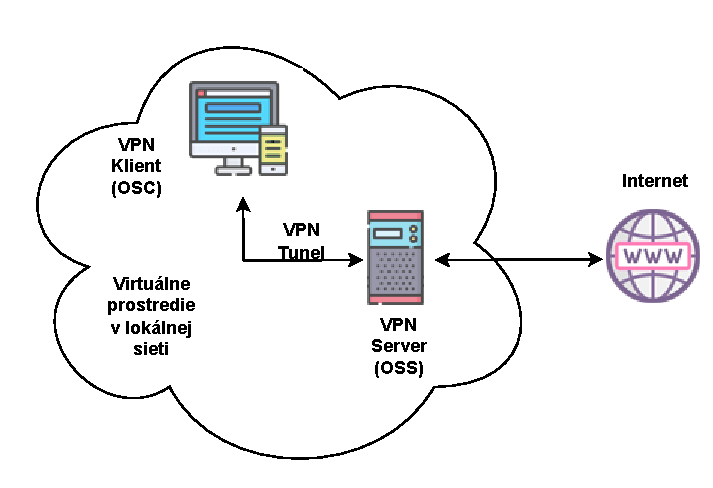
\includegraphics[width=0.9\textwidth]{figures/vpnsimple}
	\caption{Schéma jednoduchej VPN}
	\label{vpnsimple}
\end{figure}

DSVPN používa protokol riadenia prenosu -- \acrshort{tcp} \cite{tcp}. Medzi ďalšie pozitíva patrí:
\begin{itemize}
	\item{Používa iba modernú kryptografiu s formálne overenými implementáciami.}
	\item{Malá a konštantná pamäťová stopa. Nevykonáva žiadne dynamické alokovanie pamäte (z ang. \textit{heap memory}).}
	\item{Malý (~25 KB) a čitateľný kód. Žiadne vonkajšie závislosti (z ang. \textit{Dependencies}).}
	\item{Funguje po preklade GCC prekladačom. Bez dlhej dokumentácia, žiaden konfiguračný súbor, dodatočná konfigurácia. DSVPN je spustiteľná jednoriadkovým príkazom na serveri, obdobne na klientovi. Bez potreby konfigurácie brány firewall a pravidiel smerovania.}
	\item{Funguje na Linuxe (kernel $\geq$ 3.17), macOS a OpenBSD, DragonFly BSD, FreeBSD a NetBSD v klientskych a point-to-point režimoch. Pridanie podpory pre iné operačné systémy je triviálne.}
	\item{Nedochádza k úniku IP medzi pripojeniami, ak sa sieť nezmení. Blokuje IPv6 na klientovi, aby sa zabránilo úniku IPv6 adries.}
\end{itemize} 

V uvedenej VPN autor zakomponoval aj možnosť pokročilejších nastavení. Celkový súhrn vstupných parametrov pri štarte programu je takýto:
\begin{lstlisting}[language=bash]
	./dsvpn   server
	<key file>
	<vpn server ip or name>|"auto"
	<vpn server port>|"auto"
	<tun interface>|"auto"
	<local tunnel ip>|"auto"
	<remote tunnel ip>"auto"
	<external ip>|"auto"

	./dsvpn   client
	<key file>
	<vpn server ip or name>
	<vpn server port>|"auto"
	<tun interface>|"auto"
	<local tunnel ip>|"auto"
	<remote tunnel ip>|"auto"
	<gateway ip>|"auto"
	\end{lstlisting} 
Väčšina parametrov je v zdrojovom kóde prednastavených na automatické hodnoty. Príkladom je port 443, vytvorenie rozhrania tun0, prevzatie externej IP adresy zo siete a ďalšie. Používateľ teda môže spúštať DSVPN pomocou príkazu s najmenej 2 parametrami v prípade servera a tromi pre prípad klienta. Dôvodom je, že klient potrebuje mať určenú IP adresu servera, na ktorý sa má pripojiť (3.parameter). Druhý parameter v poradí je už spomenutá cesta k zdieľanému 256-bitovému kľúču.   

\section{Kryptografia použitá v DSVPN}
DSVPN používa v svojej implementácií malú sebestačnú kryptografickú knižnicu -- \textit{Charm}\footnote{\url{https://github.com/jedisct1/charm}}. Jej autorom je tvorca DSVPN. Implementácia umožňuje autentizované šifrovanie (z ang.\textit{authenticated encryption}) a hašovanie kľúčov (z ang. \textit{keyed hashing}). Správnosť implementácie algoritmu v knižnici programátor overil pomocou nástroja \textbf{Cryptol}\footnote{\url{https://cryptol.net/index.html}}. Uvedený nástroj slúži na zápis algoritmu do matematickej špecifikácií. Tým poskytne možnosť jednoduchšej a hlavne korektnej implementácie zvoleného kryptografického algoritmu. Zároveň je možné program využiť aj na verifikáciu vytvoreného riešenia. Obdobne sú v repozitári knižnice ponechané overovacie skripty pre jednoduché spustenie. 

Kryptografický algoritmus použitý v DSVPN je Xoodoo permutácia v duplex móde, pričom môže byť jednoducho nahradená napríklad Gimli-im\footnote{\url{https://github.com/jedisct1/gimli}} \cite{gimli} alebo Simpira384\footnote{\url{https://github.com/jedisct1/simpira384}} \cite{simpira}. Pri zmene musí používateľ zasiahnuť do zdrojového kódu v súbore \textbf{charm.c}, ktorého obsahom sú kryptografické primitíva.     
\section{Experimentálne overenie VPN}
DSVPN sme prakticky overili pomocou dvojice virtuálnych strojov OSS a OSC, ktorých opis je obsahom \ref{merania}. Na zariadení OSS sme pomocou balička make a GCC prekladača vykonali inštaláciu DSVPN. Obdobný postup je aplikovaný aj vo VM OSC. Na OSS spúšťame VPN Server, ktorý nám poskytne IP adresu, prostredníctvom ktorej budeme komunikovať s vonkajším svetom. Na spustenie a vytvorenie spojenie vykonáme nasledujúce úkony:
\begin{enumerate}
	\item Vygenerovanie zdieľaného kľúča:\begin{lstlisting}[language=bash]
		dd if=/dev/urandom of=vpn.key count=1 bs=32
	\end{lstlisting} 
-- zdieľaný kľúč, ktorý sme vygenerovali, sa nám uložil do súboru \textit{vpn.key}. Jeho veľkosť je 32 bajtov, teda 256 bitov. Kľúč je potrebné vložiť do priečinka s programom \textit{dsvpn} v oboch zariadeniach -- OSS aj OSC alebo zadať cestu ako parameter, kde sa kľúč nachádza.
	\item OSS zariadenie: \begin{lstlisting}[language=bash] 
	sudo ./dsvpn server vpn.key auto 
	2340 auto 10.8.0.254 10.8.0.2
	\end{lstlisting} 
-- tento príkaz zabezpečí spustenie VPN servera na prostredí OSS s IP adresou. Príkaz \lstinline|sudo| nám spustí program s administrátorskými právami. Piaty parameter nastavuje IP adresu servera. V našom prípade \lstinline|auto|, použije aktuálne používanú IP na komunikáciu s vonkajším prostredím. Príkazom ďalej definujeme portové číslo 2340, ktoré sa použije pri nastolení TCP spojenie medzi klientom a serverom. Poslednou konfiguráciou je priradenie mena a IP adresy tunelov, ktoré bude využívať naše zariaadenie -- 10.8.0.254 a druhý koniec tunela -- 10.8.0.2. Používateľ má ešte možnosť nastaviť tzv. External IP. Tú by sme využili ak by sme spúšťali DSVPN na routri poskytovateľa internetu. Obdobne na klientovi vieme nastaviť gateway IP, ktorá slúži na presmerovanie komunikácie k serveru. Po spustení príkazu si vieme overiť našu konfiguráciu\footnote{Pomocou \lstinline|ip address show tun0| overíme IPv4 adresu VPN tunela.}. 
	\item OSC zariadenie: \begin{lstlisting}[language=bash] 
	sudo ./dsvpn client vpn.key 192.168.88.62 
	2340 auto 10.8.0.2 10.8.0.254
	\end{lstlisting} 
-- uvedený príkaz zabezpečí, že sa pripojíme na VPN Server, ktorý ma ip adresu \textit{192.168.88.62} s portom 2340. Následne vzniká TCP spojenie. Dôležité je si všimnúť poradie adries tunelov. Je opačné ako v prípade servera. 
	\item V prípade úspešnej konektivity sa operácia podarila a pre okolitý svet sme viditelný pomocou IP adresy, ktorú sme zvolili. 
\end{enumerate}

Na overenie správnosti funkcionality nám postačí jednoduchý sieťový príkaz \lstinline|traceroute|. Napríklad \lstinline|traceroute google.sk|\footnote{vo Windows CMD prostredí: \lstinline|tracert google.sk|}. Prvá z uvedených adries je práve tá, ktorú dané zariadenie používa. 

V našom prípade bolo nutné použiť lokálne adresy vzhľadom na to, že obe VM bežia na jednom hosťovskom počítači. Obidva zariadenia sú tým pádom pripojené k jednému internetovému poskytovateľovi, čo má za následok takmer rovnaké smerovanie k vzdialenej doméne. 

Proces zistenia IP adresy VPN servera, po spustení, a overenie funkčnosti je následne znázornené pomocou \ref{ipu21},\ref{ipu20}, \ref{vpntru20}.
V  \ref{ipu21} sme žltou farbou znázornili IP adresu, na ktorej je VPN server dostupný. Oranžová farba znázorňuje IP adresy tunelu medzi serverom a klientom v tomto poradí. Následne v \ref{ipu20} môžeme vidieť to isté pre klienta.
  \begin{figure}
  	\centering
  	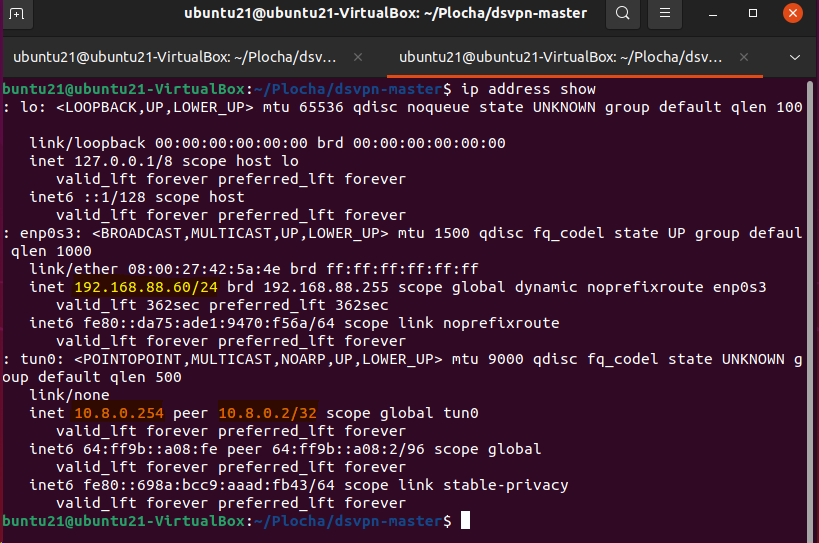
\includegraphics[width=0.9\textwidth]{figures/ipu21}
  	\caption{Zistenie IP adries VPN Servera na VM OSS}
  	\label{ipu21}
  \end{figure}
  

\begin{figure}
	\centering
	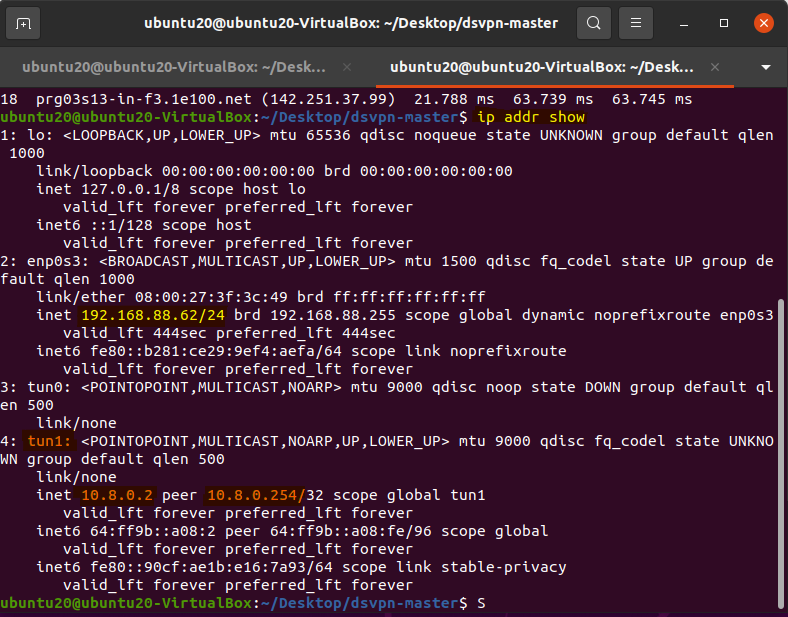
\includegraphics[width=0.9\textwidth]{figures/ipu20}
	\caption{Zistenie IP adries VPN Klienta na VM OSC}
	\label{ipu20}
\end{figure}
Nakoniec, v \ref{vpntru20} môžeme vidieť ako klient pri internetovej komunikácií používa namiesto svojej vlastnej, adresu poskytnutú VPN Serverom na zariadení OSS -- žltou zvýraznená IP. Červenou je zaškrnutá farba poskytovateľa internetu. 

\begin{figure}
	\centering
	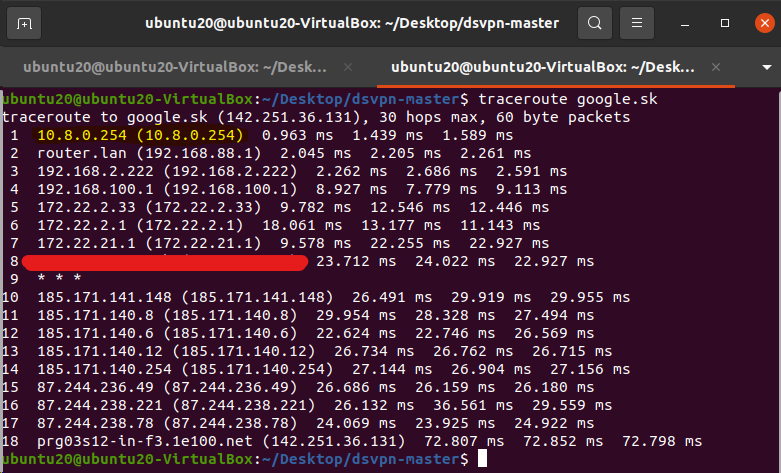
\includegraphics[width=0.9\textwidth]{figures/vpntru20}
	\caption{Overenie funkcionality DSVPN pomocou traceroute}
	\label{vpntru20}
\end{figure}
\section{Princíp fungovania programu}
DSVPN vytvára VPN sieť medzi VPN klientom a VPN serverom. Na obidvoch zariadeniach je potrebné spustiť program pomocou korešpondujúcich príkazov. 

Princíp vysvetlíme na praktickom príklade. Klienta umiestnime na lokálnu sieť bez prístupu na internet. Následne vymažeme všetky smerovacie pravidlá v zariadeni. Klient po tomto kroku nedokáže komunikovať so žiadným zariadením nakoľko nemá žiadne prednastavené pravidlá kam by smeroval internetovú komunikáciu. V uvedenej lokálnej sieti bude prítomný taktiež VPN server, ktorý ako jediný dokáže komunikovať s okolitým svetom. Po spustení DSVPN na obidvoch zariadeniach, dochádza k spojeniu. Jedná sa o TCP spojenie vytvorené soketmi. Úlohou soketového TCP spojenia je preposielanie už zašifrovaných dát v novom L3 pakete.  Následne DSVPN overuje stav soketov a tunelovacieho rozhrania. Ak je tun rozhranie pripravené na čítanie (obsahuje pakety), tak dochádza k ich spracovaniu (šifrovaniu) a preposlaní cez soket. Po prijatí sa dáta dešifrujú a smerujú na základe dát z L3 IP hlavičky. 

Toto je celý princíp zabezpečenej komunikácie medzi Klientom a Serverom vo VPN sieti na L3 vrstve. Aby sme docielili plnohodnotnú funkcionalitu VPN, tak potrebujeme do tohto riešenia zakomponovať smerovanie. Tým, že dáta smerujeme von z tejto siete, tak je ešte potrebné upraviť niektoré systémové smerovacie pravidla.      

Okrem načrtnutého príkladu s prístupom na internet, dokáže klient takto získať konektivitu k jemu nedostupným segmentom siete. Samozrejme za predpokladu, že sú dostupné pre server. Ako príklad môže byť diskové úložisko. Prípadne prístup na internetové domény. V angličtine sa takýto termín označuje ako \textit{remote access}, teda vzdialený prístup. Je to tiež veľmi obľúbený a používaný typ VPN siete. 

Funkcionalita DSVPN je znázornená pomocou schémy \ref{dsvpnarch}. V nej môžeme na ľavej strane vidieť čo sa deje s paketom pri požiadavke smerom od VPN klienta k VPN serveru. OS na základe požiadavky formoju L3 pakety. Po presmerovaní paketu na tunel DSVPN zašifruje tieto dáta. Následne ich zapíše na soket, ktorý tvorí so serverom TCP spojenie. Server tieto dáta spracuje a vykoná potrebné náležitosti. Po získaní odpovede zasa Server odpovedá klientovi rovnakým mechanizmom. Čitateľovi by som rád doplnil, že v schéme sme pre DSVPN vytvorili 2 bloky. \textbf{DSVPN IN} a \textbf{DSVPN OUT}. Funkcionalita je znázornená iba v spodnej časti schémy. Jedná sa však o identické bloky.
% TODO: \usepackage{graphicx} required
\begin{figure}[h!]
	\centering
	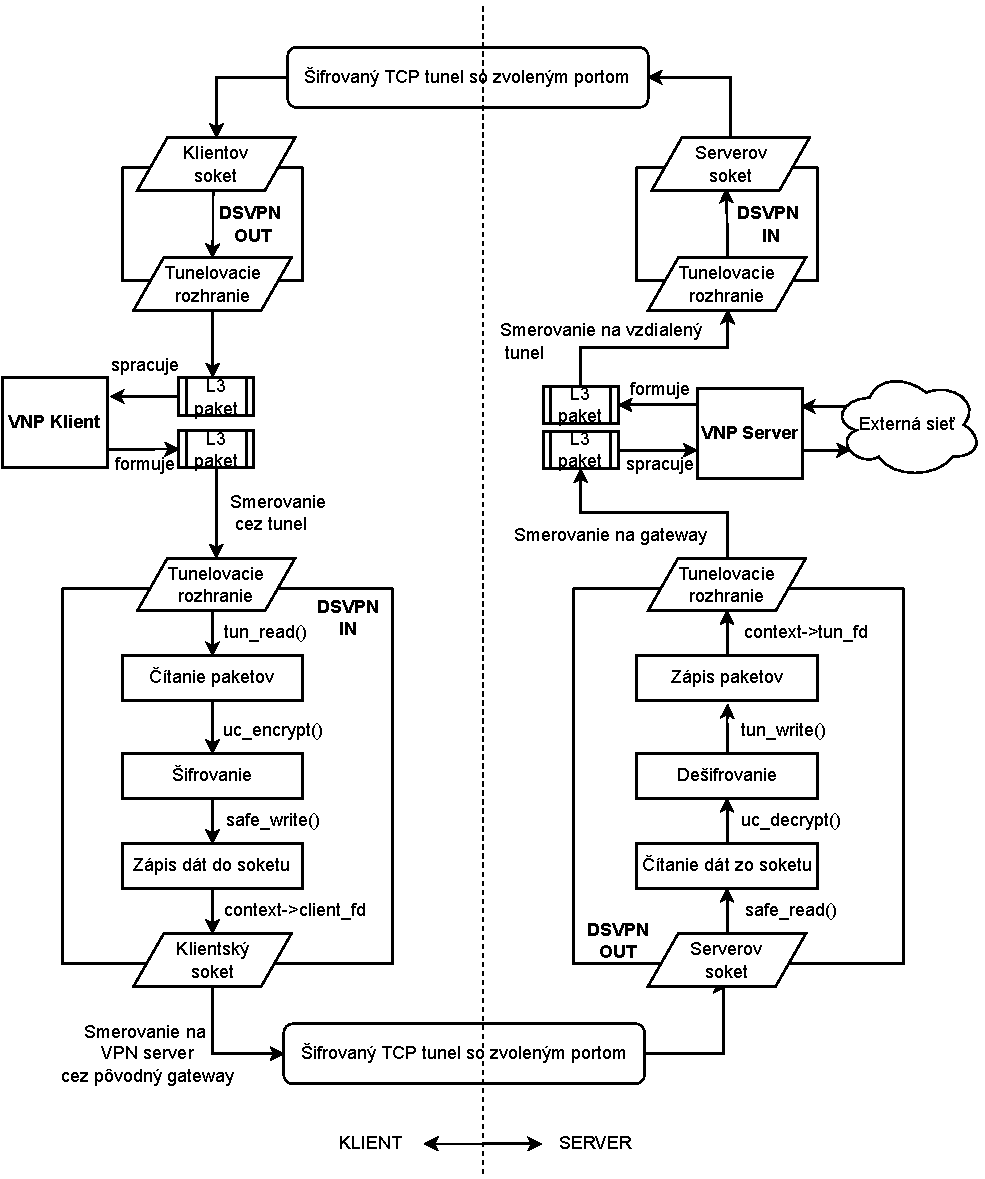
\includegraphics[width=1.1\textwidth]{figures/dsvpn.pdf}
	\caption{Ukážka prenosu paketu naprieč DSVPN}
	\label{dsvpnarch}
\end{figure}


 
\section{Analýza zdrojového kódu DSVPN}
Pri analýze sa zameriame výhradne na dôležité časti kódu DSVPN pre programovací jazyk C. Repozitár pozostáva z jedného make-file balíčka\cite{make}. 3 hlavičkových (.h) a k ním korešpondujúcimi zdrojovými kódmi (.c), s pomenovaním:
 \begin{enumerate}
 	\item \textbf{charm.h} -- kryptografická knižnica so 6 funkciami,
 	\item \textbf{os.h} -- funkcie čítania a zápisu paketov, vytvorenia, používania a zrušenia tunelovacieho rozhrania,
 	\item \textbf{vpn.h} -- deklarácia konštánt, endianity\cite{endianita} a niektorých závislostí OS.
 \end{enumerate}

V spomenutých hlavičkových súboroch sa nachádzajú deklarácie funkcií, ktoré VPN používa. Definície sú obsahom .c súborov, ako je v jazyku C zaužívaným zvykom. Obsahom tejto podkapitoly je analýza týchto kódov. 
 
\subsection{Súbor charm.h a charm.c}
Obsahom sú prevažne funkcie slúžiace pri behu kryptografického algoritmu XOODOO. Charm.h pozostáva z 6 funkcií. Ich implementácia nie je až tak rozsiahla. Zaberá celkovo 337 riadkov. Princípy použité v algoritme bolí opísané v kapitole 2.  
 
   \begin{minipage}{\linewidth} 	
  	\begin{lstlisting}[frame=single,
  		numbers=left,
  		caption={Obsah charm.h}\label{charm.h},
  		basicstyle=\ttfamily\small, keywordstyle=\color{black}\bfseries,]
void uc_state_init(uint32_t st[12], const unsigned char key[32], 
				  			 	 const unsigned char iv[16]);
void uc_encrypt(uint32_t st[12], unsigned char *msg, 
							  size_t msg_len, unsigned char tag[16]);	
int uc_decrypt(uint32_t st[12], unsigned char *msg, 
			   			   size_t msg_len,
			   			   const unsigned char *expected_tag, 
			   			   size_t expected_tag_len);
void uc_hash(uint32_t st[12], unsigned char h[32],
			 			 const unsigned char *msg, size_t len);
void uc_memzero(void *buf, size_t len);
void uc_randombytes_buf(void *buf, size_t len);
  		 	\end{lstlisting}
  	\end{minipage}\\
Z názvov funkcií je pomerne jasné čo sa v jednotlivých volaniach deje.   
 \subsection{Súbor os.h a os.c}
Obsahom su funkcie, ktorých úlohami sú čítanie alebo pridanie \acrshort{gw}, vytvorenie a nastavenie tunelu v danom OS. Následne je aplikovaná úprava firewall pravidiel, tak aby všetka komunikácia bola presmerovaná na VPN server. Úprava firewall pravidiel je závislá od role, pod ktorou je VPN spustená. Teda či sa jedná o server alebo klienta. 
Celkovo je obsahom 12 funkcií, ktoré riešia uvedené úlohy. Detail je možné vidiet v \ref{os.h}.
 
 \begin{minipage}{\linewidth} 	
	\begin{lstlisting}[frame=single,
		numbers=left,
		caption={Obsah ZK os.h}\label{os.h},
		basicstyle=\ttfamily\small, keywordstyle=\color{black}\bfseries,]
 ssize_t safe_read(const int fd, void *const buf_, size_t count, 
 						       const int timeout);
 ssize_t safe_write(const int fd, const void *const buf_, 
 							      size_t count,
 							      const int timeout);
 ssize_t safe_read_partial(const int fd, void *const buf_,
 							 					   const size_t max_count);
 ssize_t safe_write_partial(const int fd, void *const buf_, 
 							    		     	const size_t max_count);
 
 typedef struct Cmds {
 	const char *const *set;
 	const char *const *unset;
 } Cmds;
 
 Cmds firewall_rules_cmds(int is_server);
 int shell_cmd(const char *substs[][2], const char *args_str,
 			         int silent);
 const char *get_default_gw_ip(void);
 const char *get_default_ext_if_name(void);
 int tcp_opts(int fd);
 int tun_create(char if_name[IFNAMSIZ], const char *wanted_name);
 int tun_set_mtu(const char *if_name, int mtu);
 ssize_t tun_read(int fd, void *data, size_t size);
 ssize_t tun_write(int fd, const void *data, size_t size); 
\end{lstlisting}
\end{minipage}\\ 
Samozrejmosťou je implementácie čítania a zápisu dát z TUN tunelu, soketu a príkazového riadku. 
 \subsection{Súbor vpn.h a vpn.c}
 Hlavičkový súbor obsahuje prevažne definovanie niektorých parametrov potrebných na správnu funkcionalitu VPN, spoločne s korekciou pre niektoré OS. Viď. \ref{vpn.h}. Ostatné parametre, ktoré bolí opísané pre spustenie, su definované práve v tomto súbore (porty, IP adresy, MTU atď.).
 
 \begin{minipage}{\linewidth} 	
 	\begin{lstlisting}[frame=single,
 		numbers=left,
 		caption={Obsah ZK vpn.h}\label{vpn.h},
 		basicstyle=\ttfamily\small, keywordstyle=\color{black}\bfseries,]
 /*UNIX-like OS Dependent Libraries*/
 #include <sys/ioctl.h>
 #include <sys/socket.h>
 #include <sys/types.h>
 #include <sys/uio.h>
 #include <sys/wait.h>
 #include <net/if.h>
 #include <netinet/in.h>
 #include <netinet/tcp.h>
 /*End UNIX-like OS Dependent Libraries*/
 /*OS setup dependencies*/
 #ifdef __linux__
 #include <linux/if_tun.h>
 #endif
 
 #ifdef __APPLE__
 #include <net/if_utun.h>
 #include <sys/kern_control.h>
 #include <sys/sys_domain.h>
 #endif
 
 #ifdef __NetBSD__
 #define DEFAULT_MTU 1500
 #else
 #define DEFAULT_MTU 9000
 #endif
 /*End of OS setup dependencies*/ 
 	\end{lstlisting}
\end{minipage}\\

\subsubsection{Main() -- Beh programu}
Pred samotným opisom by som rád upozornil na jeden fakt. Autor DSVPN používa vo veľkej miere zápis pomocou tzv. ternárnych operátorov. Viac informácií o tejto problematike je možné nájsť v \cite{ternary}. V skratke, používa sa podmienený zápis hodnoty do premennej.

Vpn.c je hlavným zdrojovým kódom DSVPN. V jeho vnútri nájdeme hlavnú, štartovaciu, funkciu main. Zároveň má prilinkované aj vyššie uvedené knižnice. Ako prvé dochádza k inicializácií premennej štruktúry \lstinline|Context|\ref{context}. Štruktúra v sebe nesie všetky premenné, potrebné na správne fungovanie programu.

\begin{minipage}{\linewidth} 	
	\begin{lstlisting}[frame=single,
		numbers=left,
		caption={Štruktúra Context}\label{context},
		basicstyle=\ttfamily\small, keywordstyle=\color{black}\bfseries,]
typedef struct Context_ {
	const char *  wanted_if_name;
	const char *  local_tun_ip;
	const char *  remote_tun_ip;
	const char *  local_tun_ip6;
	const char *  remote_tun_ip6;
	const char *  server_ip_or_name;
	const char *  server_port;
	const char *  ext_if_name;
	const char *  wanted_ext_gw_ip;
	char          client_ip[NI_MAXHOST];
	char          ext_gw_ip[64];
	char          server_ip[64];
	char          if_name[IFNAMSIZ];
	int           is_server;
	int           tun_fd;
	int           client_fd;
	int           listen_fd;
	int           congestion;
	int           firewall_rules_set;
	Buf           client_buf;
	struct pollfd fds[3];
	uint32_t      uc_kx_st[12];
	uint32_t      uc_st[2][12];
} Context;   
 	\end{lstlisting}
\end{minipage}\\ 

 Následne dochádza k načítaniu vopred zdieľaného kľúča pomocou pomocnej funkcie 
\\
 \lstinline|load_key_file()|\ref{load}. Úlohou je prečítanie kľúča, pričom sa používa funkcia z os.c -- \lstinline|safe_read()|. Realizuje sa znakové spočítanie, v ktorom je zakomponovaná funkcia  \lstinline|poll()| \cite{poll}. Dôvodom je, že \lstinline|safe_read()| sa používa aj pri čítaní zo soketu a~tunelu. V linuxe je čítanie z týchto typov rovnaké. Tato časť kódu je však podmienená špecifickou chybou, ktorú je možné dostať len pri čítaní soketu, respektíve tunelu.  
 V prípade, ak sa prečítalo 32 bajtov, \lstinline|safe_read()| vracia 0. Následne sa inicializuje stav v XOODOO.
 
 \begin{minipage}{\linewidth} 	
 	\begin{lstlisting}[frame=single,
 		numbers=left,
 		caption={Načítanie zdieľaného kľúča}\label{load},
 		basicstyle=\ttfamily\small, keywordstyle=\color{black}\bfseries,]
 static int load_key_file(Context *context, const char *file)
 {
 	unsigned char key[32];
 	int           fd;
 	
 	if ((fd = open(file, O_RDONLY)) == -1) {
 		return -1;
 	}
 	if (safe_read(fd, key, sizeof key, -1) != sizeof key) {
 		(void) close(fd);
 		return -1;
 	}
 	uc_state_init(context->uc_kx_st, key, 
 							 (const unsigned char *) "VPN Key Exchange");
 	uc_memzero(key, sizeof key);
 	
 	return close(fd);
 }
  	\end{lstlisting}
\end{minipage}\\ 
Ako môžeme vidieť v implementácii sú bežne použité smerníky. Vo výsledku, tak dokážeme preniesť zmenu hodnôt na viaceré premenné.
 
V prípade, ak používateľ pri štarte nezmenil parameter pre IP adresu sieťovej brány\footnote{z ang. \textit{GateWay}} (ďalej \acrshort{gw}), tak sa používa pôvodná. Tá sa získa pomocou funkcie \\\lstinline|get_default_gw_ip()|, ktorá je deklarovaná v \ref{os.h}. Prostredníctvom shell príkazu \lstinline|ip route| a \lstinline|read_from_shell_command()| funkcie, dochádza k extrakcii informácií priamo z príkazového riadka. Tento krok je teda závislý od \acrshort{os}, v ktorom používateľ pracuje. Nasleduje overenie návratových hodnôt z funkcií iba v prípade ak je DSVPN spustené ako Klient.
 
Program v prípade servera pokračuje s \lstinline|get_default_ext_if_name()|. \\Obdobne ako v predchádzajúcom odstavci je realizácia funkcionality, vykonaná pomocou terminálu. Podstata spočíva v zistení mena tunelovacieho rozhrania.
 
Po nastavení parametrov sa dostávame k vytvoreniu tunelovacieho rozhrania. V tomto kroku autor používa funckiu \lstinline|tun_create|. Úloha je vysoko závislá od OS. Dôsledkom toho je možné vidieť vetvenie funkcionality vzhľadom k bežiacemu OS. DSVPN poskytuje kompatibilitu pre 6 OS, medzi, ktoré patrí Linux, FreeBSD, NetBSD, OpenBSD, MacOS, DragonFly. Následne na základe systému dochádza k vytváraniu tunelu s prednastaveným, resp. zvoleným menom. Program ďalej nastaví maximálnu veľkosť prepravovaného paketu\footnote{z ang. \textit{Maximum Transmission Unit}} (ďalej \acrshort{mtu}) na 1500/9000 bajtov. 
 
Po príprave tunelu dochádza k overeniu dostupnosti VPN servera. Tento krok vykonáva funkcia \lstinline|resolve_ip|. Tá ma v sebe vnorené 2 funkcie, ktoré su menným ekvivalentom aj vo Windows knižniciach. Jedná sa o funkcie \lstinline|getaddrinfo| a \lstinline|getnameinfo|.  
 
Posledným krokom súvisiacim s konfiguráciou prostredia je vytvorenie pravidla pre branu FireWall (ďalej \acrshort{fw}). Tento úkon realizuje \lstinline|firewall_rules()|. Tento proces je opäť systémovo závislý. Jeho realizácia je vykonaná pomocou globálne definovanej funkcie \lstinline|Cmds firewall_rules_cmds()|. Tá obsahuje súbor prednastavených príkazov. Ich úlohou je presmerovanie celej premávky cez vzniknutý tunel.
 
Posledným úkonom je samotný beh VPN. Ten spúšťa funkcia \lstinline|doit()|. Doterajší beh programu je jednoducho znázornený pomocou flow diagramu \ref{fc1}.
 
\begin{figure}
	\centering
	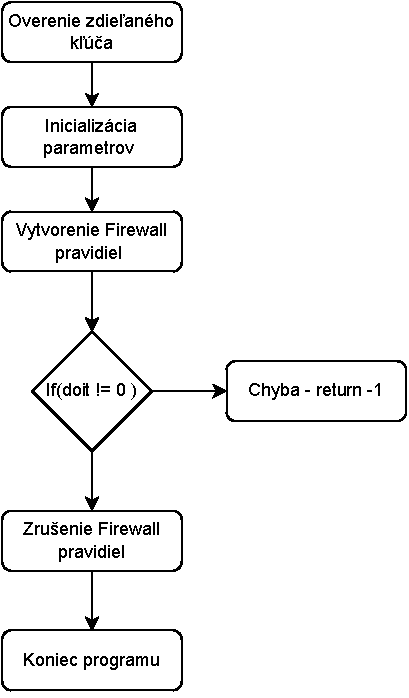
\includegraphics[width=0.6\textwidth]{figures/fc1}
	\caption{Schéma behu DSVPN vo funkcii main()}
	\label{fc1}
\end{figure}

Od tohto momentu sa presúvame k postupnému vnáraniu do procesu spojenia a spracovania dát. Hlavnou úlohou funkcie \lstinline|doit()| je nadviazanie soketového TCP spojenia medzi klientom a serverom. Vo vnútri \lstinline|doit()| preto dochádza k vetveniu programu. V prípade, že je DSVPN spustená ako server spustí sa funkcia \lstinline|tcp_listener()|. V opačnom prípade \lstinline|client_reconnect()|. Listener vytvára socket a následne pomocou systemovej funkcie \lstinline|bind()| sa napojí na zvolený port. Potom čaká na spojenie od klienta pomocou funkcie \lstinline|listen()|. Smerník na socket je uložený do smerníka na štruktúru Context.
Klient používa vetvu s~\lstinline|Client_reconnect()|. V nej sa snaží opakovane nadviazať spojenie so serverom. Za týmto účelom \lstinline|client_connect()|. Pred týmto úkonom samozrejme dochádza k overeniu či už nedošlo k nadviazaniu spojenia. O to sa stará \\\lstinline|client_disconnect()|, ktorý ruší aktívne spojenie.

\lstinline|Client_connect()| slúži na pripojenie klienta k serveru. Vykonáva aj úpravu pravidiel v \acrshort{fw}. Následne sa pokúša o nadviazania spojenia pomocou funkcie  \lstinline|tcp_client()|. Po tejto sérií úloh sa vraciame opäť do \lstinline|doit()|. V cykle \lstinline|while| sa vykonávaná funkcia \lstinline|event_loop()|, v ktorej dochádza k použitiu kryptografickej knižnice charm. Jej obsahom je inicializácia pomocných premenných. viď. zdrojový kód \ref{el}. Schéma \ref{fc2} znázorňuje doteraz opísané skutočnosti.
  
  \begin{minipage}{\linewidth} 	
  	\begin{lstlisting}[frame=single,
  		numbers=left,
  		caption={Premenné funkcie event loop}\label{el},
  		basicstyle=\ttfamily\small, keywordstyle=\color{black}\bfseries,]
  struct pollfd *const fds = context->fds;
  Buf                  tun_buf;
  Buf *                client_buf = &context->client_buf;
  ssize_t              len;
  int                  found_fds;
  int                  new_client_fd;
    	\end{lstlisting}
\end{minipage}\\ 
 
 

\begin{figure}
	\centering
	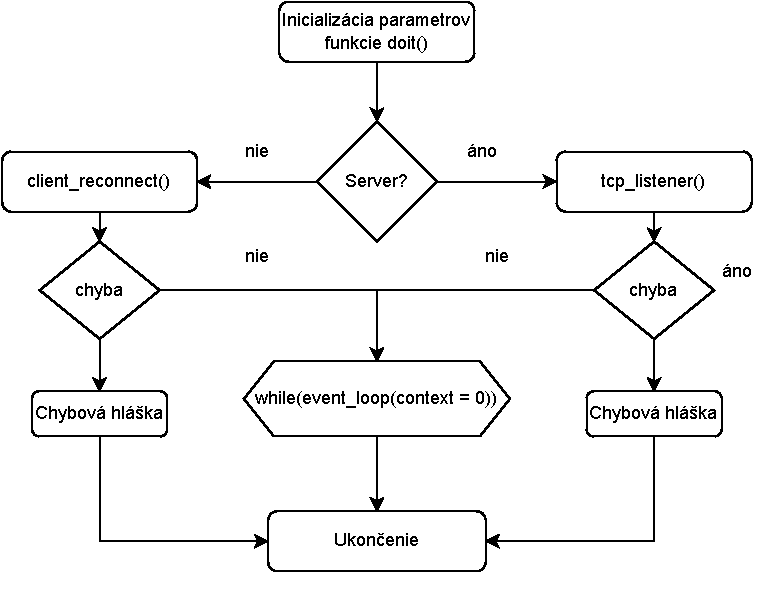
\includegraphics[width=0.9\textwidth]{figures/fc2}
	\caption{Princíp fungovania funkcie doit()}
	\label{fc2}
\end{figure}

\subsubsection{Funckia \lstinline|event_loop()|}
\lstinline|Event_loop()| je 111 riadkov dlhá funkcia. Jej obsah môžeme rozdeliť na overovací a výkonový. Úlohou niekoľkých \lstinline|if-ov| vo funkcii je preverovanie signálov, spätných hodnôt a podobných premenných, ktoré by signalizovali chybu, používateľov záujem o ukončenie programu alebo signál pre čítanie dát zo soketov, respektíve tunelov. 
 
Zaujímavé je taktiež predom definované makro \lstinline|BUFFERBLOAT_CONTROL|. Jeho úlohou je zamedzenie problému zvaného \textbf{Bufferbloat}. V skratke, je to nechcený jav, ktorý je zapríčinený nadmerným ukladaním paketov do vyrovnávacej pamäte, tzv. zahltenie. To ma za následok vysokú latenciu a tzv. z ang. \textit{Packet Delay Variation} (ďalej \acrshort{pdv}/Jitter), v paketovo-orientovaných sieťach. Viac o tejto problematike je možne si prečítať na \cite{bufferbloat}.
 
Na druhej strane výkonové funkcie, ako hovorí ich názov. niečo vykonávajú. Do tejto kategórie sme zaradili funkcie:
 \begin{itemize}
 	\item\lstinline|tcp_accept()| -- slúži na nastolenie nového soketového TCP spojenia s klientom, 
 	\item\lstinline|tun_read()| -- v prípade linuxového OS, volá \lstinline|safe_read_partial()| na zapísanie dát do nami vytvoreného tunelovacieho rozhrania,
 	\item\lstinline|uc_encrypt()| -- kryptografické šifrovanie paketov z tunelovacieho rozhrania,
 	\item\lstinline|safe_write_partial()| -- používa štandardizovanú funkciu \lstinline|write()| vo while cykle, zapíše zašifrované dáta do buffera určeného pre odoslanie klientovi, vracia počet zapísaných dát,
 	\item\lstinline|safe_write()| -- používa sa v prípade ak došlo k zahlteniu paketmi,
 	\item\lstinline|client_reconnect()| -- slúži na obnovu spojenia v prípade chyby,
 	\item\lstinline|safe_read_partial()| -- obdobne ako pri \lstinline|write()|, používa \lstinline|read()| funkciu,
 	\item\lstinline|uc_decrypt()| -- kryptografické dešifrovanie správy a následne odoslanie na tunelovacie rozhranie,
 	\item\lstinline|tun_write()| -- volá \lstinline|safe_write| pri OS Linux, teda klasický zápis dešifrovaných dát.
 \end{itemize}
Metóda použitá pri zápise zašifrovaných dát vo funkcii \lstinline|event_loop()| je znázornená v \ref{ed}.

 \begin{minipage}{\linewidth} 	
 	\begin{lstlisting}[frame=single,
 		numbers=left,
 		caption={Spôsob zápisu šifrovaných dát}\label{ed},
 		basicstyle=\ttfamily\small, keywordstyle=\color{black}\bfseries,]
 		
 writenb = safe_write_partial(context->client_fd, tun_buf.len,
 			    	 		         		  2U + TAG_LEN + len); 
 if (writenb < (ssize_t) 0) {// kontrola zahltenia -- bufferbloat
 	context->congestion = 1; 
 	writenb             = (ssize_t) 0;
 }
// ak doslo k zahlteniu
 if (writenb != (ssize_t)(2U + TAG_LEN + len)) {
 	writenb = safe_write(context->client_fd, tun_buf.len + writenb,
 	2U + TAG_LEN + len - writenb, TIMEOUT); 
 }
   	\end{lstlisting}
\end{minipage}\\ 
V princípe celá logika tejto VPN pozostáva z kontroly obsahu tunelovacieho rozhrania a aktívnych soketov. Následne ak sa na vstupoch nachádzajú dáta dochádza k ich čítaniu, dešifrovaniu a následnému odoslaniu dát aplikácií, ktorej prislúchajú.

Na konci funkcie \lstinline|event_loop()| sa nachádza ešte overenie pre prípad keď buffer s dátami nie je úplne plný. V tomto prípade funkcia vykonáva posun uložených bajtov na začiatok buffera. Inými slovami pripravuje dáta na ďalšie čítanie. Vyššie uvedené výroky sú znázornené v zdrojovom kóde \ref{bufferPreparation}.

\begin{lstlisting}[frame=single,
	numbers=left,
	caption={Príprava dát na ďalšie čítanie}\label{bufferPreparation},
	basicstyle=\ttfamily\small, keywordstyle=\color{black}\bfseries,]
	
	if (2 + TAG_LEN + MAX_PACKET_LEN != len_with_header) { 
		unsigned char *rbuf      = client_buf->len;
		size_t         remaining = client_buf->pos - len_with_header;
		memmove(rbuf, rbuf + len_with_header, remaining);
	}
	client_buf->pos -= len_with_header;
\end{lstlisting}
 
\subsubsection{Šifrovanie a dešifrovanie}
Proces šifrovanie resp. dešifrovania správy nastáva na oboch stranách spojenia, teda pri klientovi aj serveri. Zdrojový kód \ref{SS} demonštruje šifrovanie implementované v funkcii \lstinline|uc_encrypt()|. Tento proces sme sa pokúsili opísať v grafe \ref{fc3}. 

\begin{figure}
	\centering
	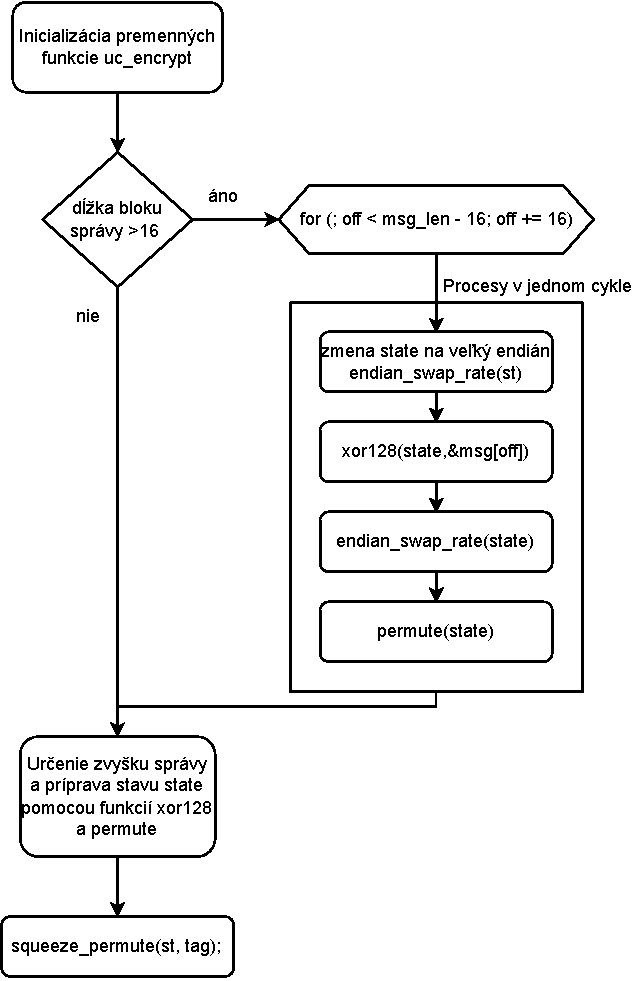
\includegraphics[width=0.8\textwidth]{figures/fc3}
	\caption{Proces šifrovania v funkcii uc\_encrypt()}
	\label{fc3}
\end{figure}

\begin{minipage}{\linewidth} 	
	\begin{lstlisting}[frame=single,
		numbers=left,
		caption={Šifrovanie správy pomocou uc\_encrypt}\label{SS},
		basicstyle=\ttfamily\small, keywordstyle=\color{black}\bfseries,]
 		
void uc_encrypt(uint32_t st[12], unsigned char *msg, 
					      size_t msg_len, unsigned char tag[16])
{	//spracovanie po 16 znakov
	unsigned char squeezed[16];
	unsigned char padded[16 + 1];
	size_t        off = 0;
	size_t        leftover;
	
	if (msg_len > 16) {
		for (; off < msg_len - 16; off += 16) {
			endian_swap_rate(st);
			memcpy(squeezed, st, 16);
			xor128(st, &msg[off]);
			endian_swap_rate(st);
			xor128(&msg[off], squeezed);
			permute(st);
		}
	}
	leftover = msg_len - off;
	memset(padded, 0, 16);
	mem_cpy(padded, &msg[off], leftover);
	padded[leftover] = 0x80;
	endian_swap_rate(st);
	memcpy(squeezed, st, 16);
	xor128(st, padded);
	endian_swap_rate(st);
	st[11] ^= (1UL << 24 | (uint32_t) leftover >> 4 << 25
				    | 1UL << 26); 
	xor128(padded, squeezed);
	mem_cpy(&msg[off], padded, leftover);
	permute(st);
	squeeze_permute(st, tag);		//vytvorenie tagu
}
  	\end{lstlisting}
\end{minipage}\\ 

Ako je viditeľne v kóde dochádza k častému použitiu 2 funkcií. Nimi sú  \lstinline|xor128()| a  \lstinline|permute()|. Jedná sa o pomerne dôležité bloky pre správne fungovanie šifrovacieho algoritmu. Obsah prvej z uvedených je preto znázornený v zdrojovom kóde \ref{xor}.

\begin{minipage}{\linewidth} 	
	\begin{lstlisting}[frame=single,
		numbers=left,
		caption={Funkcia xor128}\label{xor},
		basicstyle=\ttfamily\small, keywordstyle=\color{black}\bfseries,]
static inline void xor128(void *out, const void *in)
{
	#ifdef __SSSE3__
	_mm_storeu_si128((__m128i *) out,
	_mm_xor_si128(_mm_loadu_si128((const __m128i *) out),
	_mm_loadu_si128((const __m128i *) in)));
	#else
	unsigned char *      out_ = (unsigned char *) out;
	const unsigned char *in_  = (const unsigned char *) in;
	size_t               i;
	
	for (i = 0; i < 16; i++) {	//xororvanie jednotlivych znakov 
		out_[i] ^= in_[i];		//v 16 bitovom bloku spravy
	}
	#endif
}
  	\end{lstlisting}
\end{minipage}\\ 

Funkcia \lstinline|permute()| je pomerne rozsiahla. Jej obsah sa rozprestiera na 100 riadkoch. Jedná sa o implementáciu XOODOO permutácie, ktorá bola opísaná v kapitole číslo 2. Funkcionalita závisí od prostredia a procesorových inštrukcií. Samozrejmosťou je softvérová implementácia, ktorá je aj použitá pri behu. Dôvodom je, že naše zariadenie nemá k dispozícií uvedené procesorové inštrukcie. Blok, ktorý je použitý pri volaní sa nachádza v \ref{permute}.   

\begin{minipage}{\linewidth} 	
	\begin{lstlisting}[frame=single,
		numbers=left,
		caption={Funkcia Permute + makrá }\label{permute},
		basicstyle=\ttfamily\small, keywordstyle=\color{black}\bfseries,]
#define ROTR32(x, b) (uint32_t)(((x) >> (b)) | 
                     ((x) << (32 - (b))))
#define SWAP32(s, u, v)        \
do {                           \
	t      = (s)[u];             \
	(s)[u] = (s)[v], (s)[v] = t; \
} while (0)
	
static void permute(uint32_t st[12])
{
	uint32_t e[4], a, b, c, t, r, i;	
	for (r = 0; r < XOODOO_ROUNDS; r++) {
		for (i = 0; i < 4; i++) {
			e[i] = ROTR32(st[i] ^ st[i + 4] ^ st[i + 8], 18);
			e[i] ^= ROTR32(e[i], 9);
		}
		for (i = 0; i < 12; i++) {
			st[i] ^= e[(i - 1) & 3];
		}
		SWAP32(st, 7, 4);
		SWAP32(st, 7, 5);
		SWAP32(st, 7, 6);
		st[0] ^= RK[r];
		for (i = 0; i < 4; i++) {
			a         = st[i];
			b         = st[i + 4];
			c         = ROTR32(st[i + 8], 21);
			st[i + 8] = ROTR32((b & ~a) ^ c, 24);
			st[i + 4] = ROTR32((a & ~c) ^ b, 31);
			st[i] ^= c & ~b;
		}
		SWAP32(st, 8, 10);
		SWAP32(st, 9, 11);
	}	
}
	\end{lstlisting}
\end{minipage}\\
Na druhej strane k \textbf{dešifrovaniu} dochádza v momente ak sa v klientskom sokete nachádzajú dáta. Program overuje či sú v premennej \lstinline|fds[POLLFD_CLIENT]| dáta určené na spracovanie. \lstinline|fds[POLLFD_CLIENT]| predstavuje smerník na pamäťový blok, kde je uložený soket na druhú stranu spojenia, teda akceptovaného klienta. V momente keď sa tam nachádzajú dáta dôjde k ich čítaniu pomocou funkcie \lstinline|safe_read_partial()|. Následne program realizuje dešifrovanie funkciou \lstinline|uc_decrypt()|, ktorá je inverznou k \lstinline|uc_encrypt()|. V ukážke zdrojového kódu \ref{decrypt} a \ref{decrypt2}, si používateľ môže prezrieť obsah funkcie \lstinline|uc_decrypt()|. Po odšifrovaní dát ich program zapisuje do tunelovacieho rozhrania prostredníctvom funkcie \lstinline|tun_write()|. Následne TUN rozhranie dotvára paket a vloží ho do sieťového zásobníka\footnote{z ang. \textit{network stack}}. OS následne vykonáva ďalšie spracovanie paketu do nižších vrstiev sieťového modelu. 

\begin{minipage}{\textwidth} 	
	\begin{lstlisting}[frame=single,
		numbers=left,
		caption={Zdrojový kód funkcie na dešifrovanie správy (1.časť)}\label{decrypt},
		basicstyle=\ttfamily\small, keywordstyle=\color{black}\bfseries,]
		int uc_decrypt(uint32_t st[12], unsigned char *msg, 
		               size_t msg_len, 
		               const unsigned char *expected_tag,
		               size_t expected_tag_len)
		{
			unsigned char tag[16];
			unsigned char squeezed[16];
			unsigned char padded[16 + 1];
			size_t        off = 0;
			size_t        leftover;
			
			if (msg_len > 16) {
				for (; off < msg_len - 16; off += 16) {
					endian_swap_rate(st);
					memcpy(squeezed, st, 16);
					xor128(&msg[off], squeezed);
					xor128(st, &msg[off]);
					endian_swap_rate(st);
					permute(st);
				}
			}
			leftover = msg_len - off;
			memset(padded, 0, 16);
			mem_cpy(padded, &msg[off], leftover);
			endian_swap_rate(st);
			memset(squeezed, 0, 16);
			mem_cpy(squeezed, 
			        (const unsigned char *) (const void *) st, 
			        leftover
			        );
		    xor128(&padded, squeezed);
			padded[leftover] = 0x80;
			xor128(st, padded);
			endian_swap_rate(st);
			st[11] ^= (1UL << 24 | (uint32_t) leftover >> 4 
			<< 25 | 1UL << 26);
			mem_cpy(&msg[off], padded, leftover);
			
	\end{lstlisting}
\end{minipage}

\begin{minipage}{\textwidth} 	
	\begin{lstlisting}[frame=single,
		numbers=left,
		firstnumber=38,
		caption={Zdrojový kód funkcie na dešifrovanie správy (2.časť)}\label{decrypt2},
		basicstyle=\ttfamily\small, keywordstyle=\color{black}\bfseries,]
			permute(st);
			squeeze_permute(st, tag);
			
			if (equals(expected_tag, tag, expected_tag_len) == 0) {
				memset(msg, 0, msg_len);
				return -1;
			}
			return 0;
		}
	\end{lstlisting}
\end{minipage}\\

Pre čitateľa sme si pripravili aj názornú ukážku šifrovania a prenosu týchto dát cez soket. Za účelom ukážky použijeme už spomínaný nástroj Wireshark na zachytávanie premávky v sieťových rozhraniach. Prechod dát z pohľadu klienta medzi zariadeniami je znázornený na obrázku \ref{wiresharkpakety}. 
% TODO: \usepackage{graphicx} required
\begin{figure}[h!]
	\centering
	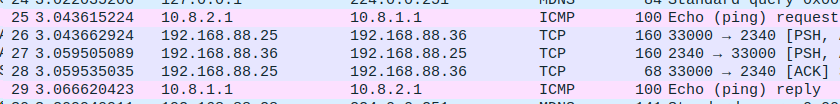
\includegraphics[width=1\textwidth]{figures/wiresharkpakety}
	\caption{Prenos zašifrovaných dát z VPN klienta na VPN server}
	\label{:wiresharkpakety}
\end{figure}
Na VPN klientovi sme spustili v príkazovom riadku jednoduchý príkaz \lstinline|ping 10.8.1.1|. Ten nám vytvára veľmi známy ICMP paket so žiadosťou o odpoveď\footnote{paket číslo 25}. Obsah tohto paketu je možné si pozrieť v obrázku \ref{req}. % TODO: \usepackage{graphicx} required
\begin{figure}[h!]
	\centering
	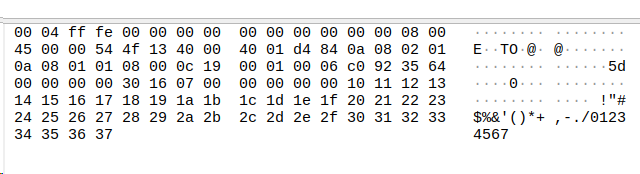
\includegraphics[width=1\textwidth]{figures/req}
	\caption{Obsah pôvodného paketu s ICMP žiadosťou}
	\label{req}
\end{figure}
Tento paket je vo VPN klinetovi po spracovaní vo DSVPN zašifrovaný pomocou XOODOO permutácie a odoslaný cez soketové TCP spojenie\footnote{paket číslo 26}. Obsah zašifrovaného paketu je znázornený v \ref{sifrovanypaket}. 
% TODO: \usepackage{graphicx} required
\begin{figure}[h!]
	\centering
	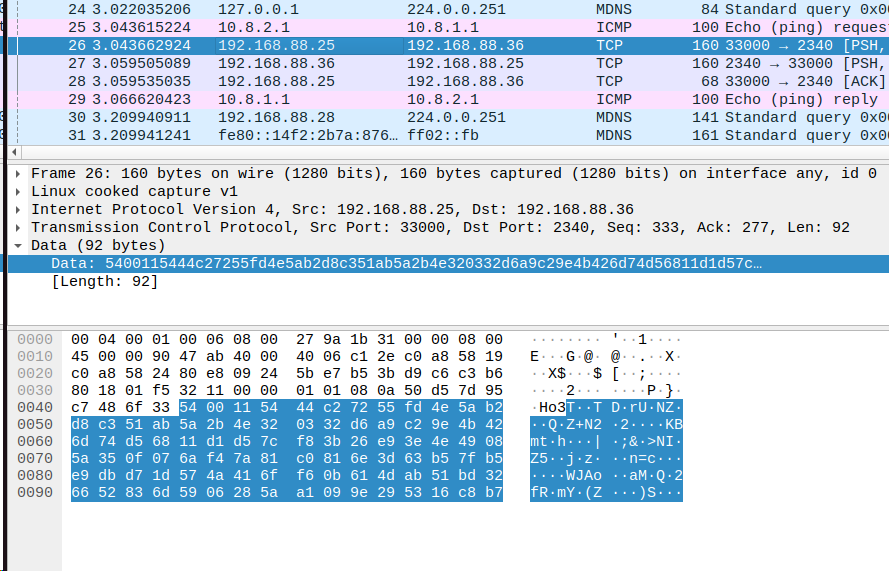
\includegraphics[width=0.9\textwidth]{figures/sifrovanypaket}
	\caption{Zašifrovaný pôvodný ICMP paket v novom TCP pakete}
	\label{sifrovanypaket}
\end{figure}
Označená časť paketu v obrázku je už spomenutý zašifrovaný ICMP paket z obrázku \ref{req}. VPN server ho po prijatí dešifruje a posiela na vlastné tunelovacie rozhranie. Odiaľ prevezme paket OS a vygeneruje odpoveď na pôvodnú požiadavku vo forme nového paketu. Ten je prenesený na klienta opäť cez soketové TCP spojenie\footnote{paket číslo 27}. Paket číslo 28 je odpoveď na úspešne prijatie. DSVPN spracuje tento paket a zapíše pôvodný na tunelovacie rozhranie.. Z hľadiska klienta už vidíme dešifrovanú odpoveď v pakete číslo 29, ktorú spracuje OS.

  
\subsubsection{Ukončenie činnosti programu}
Používateľ má možnosť ukončiť vzniknuté VPN spojenie medzi klientom a serverom pomocou jednoduchého príkazu \lstinline|crtl + c|. Program zaznamená tento vstup a ukončí cyklus. Po návrate až do hlavnej funckie \lstinline|main()| sa z OS vymažú aplikované FW pravidlá a používateľ môže používať počítač ako pred spustením DSVPN.

\section{Analýza výpočtových nárokov DSVPN}\label{analyza}
Za účelom analýzy výpočtových nárokov sme sa v práci zamerali na meranie potrebného počtu cyklov a zároveň aj času, potrebného na vykonanie šifrovanie a dešifrovanie permutacie XOODOO. Pre linuxovú platformu sme použili niektoré zabudované funkcie ako je \lstinline|clock()|. Pomocou nej sme zmerali čas vykonávania. Ukážka ako bol kód na meranie implementovaný do DSVPN je možné vidieť v ukážke zdrojového kódu
 
\begin{minipage}{\linewidth} 	
	\begin{lstlisting}[frame=single,
		numbers=left,
		caption={Ukážka spôsobu merania pri (de)šifrovaní XOODOO}\label{mneranie},
		basicstyle=\ttfamily\small, keywordstyle=\color{black}\bfseries,]
		uint64_t time,tick;	//inicializacia premennych
		clock_t t = clock();
		
		tick = cpucyclesS();
		codeTomeassure();		//funkcia urcena na meranie
		time = cpucyclesE()-tick;
		
		t = clock() - t;    //vyhodnotenie
		double time_taken = ((double)t)/CLOCKS_PER_SEC;
		printf(Size(%ld B): "%llu cycles in %f s\n", msg_length,
		       time, time_taken);	
	\end{lstlisting}
\end{minipage}\\
V prípade, ak by používateľ potreboval vykonať podobné meranie času v prostredí OS Windows, tak dávame do pozornosti tento variant. Viď zdrojový kód \ref{winmer}. Viac o použití a limitáciách je možné nájsť v práci \cite{bc}.

\begin{minipage}{\linewidth} 	
	\begin{lstlisting}[frame=single,
		numbers=left,
		caption={Meranie času vykonávania na OS Windows}\label{winmer},
		basicstyle=\ttfamily\small, keywordstyle=\color{black}\bfseries,]
	#include <windows.h>
	
	#define TIMER_INIT \	//inicializacia makra
	LARGE_INTEGER frequency; \
	LARGE_INTEGER t1,t2; \
	double elapsedTime; \
	QueryPerformanceFrequency(&frequency);

	#define TIMER_START QueryPerformanceCounter(&t1);
	#define TIMER_STOP \
	QueryPerformanceCounter(&t2); \
	elapsedTime=(double)(t2.QuadPart-t1.QuadPart)
						  /frequency.QuadPart; 	
	
	TIMER_INIT		\\pouzitie	
	{
		TIMER_START
		codeToMeasure()
	 	TIMER_STOP
 	}
	\end{lstlisting}
\end{minipage}\\

Spojenie medzi klientom a serverom je spustené na VM. Šifrovanie bolo merané na strane Klienta. Dešifrovanie sme merali v OS servera. Počas spojenia sme sa snažili naviesť stav väčšieho sieťového zataženia. Tento úkon sme zrealizovali otvorením viacerých rôznych kariet vo webovom prehliadači. Týmto spôsobom sme odsimuloval potrebu prenosu vačšieho množstva dát naprieč sieťou. Najčastejšie však do šifrovania vstupovali TCP pakety, ktoré majú za úlohu udržať soketové TCP spojenie. Ich veľkosť je 52bajtov. Z výpisu sme ešte na základe pozorovania sledovali aké veľkosti sa najčastejšie vyskytujú. Na základe takto získaných dát sme vypracovali tabuľku \ref{tabmer}. Hodnoty pre jednotlivé stĺpce boli získane ako aritmetický priemer z meraní. Pakety, ktoré vstupovali do šifrovania, resp. dešifrovania menej ako 20-krát sme z meraní vypustili. Dôvodom je snaha o získanie lepších štatistických údajov. Obdobne sme pri výpočte aritmetického priemeru nebrali do úvahy príliš veľké výchylky pri meraní počtu cyklov. Uvedené chyby merania spôsobil samotný OS, kvôli prerušovania činnosti programu DSVPN.     

\begin{table}[h!]
	\centering
	\resizebox{\textwidth}{!}{%
		\begin{tabular}{c|c|c|c|c}
			\bfseries Veľkosť dát[B] &
			\multicolumn{4}{|c}{\bfseries Názov meranej funkcie} 			
			\\
			\bfseries X &
			\multicolumn{2}{|c}{\bfseries uc\_encrypt()} &
			\multicolumn{2}{|c}{\bfseries uc\_decrypt()}
			\\
			\bfseries Počet meraní 
			& Počet cyklov
			& Čas vykonávania [s]
			& Počet cyklov
			& Čas vykonávania [s] 
			\\\hline\hline
			 52   X 1376			 
			& 1 648
			& 0.000 076
			& 2 377
			& 0.000 062
			\\		
			60  X  79	
			& 2 527
			& 0.000 049
			& 2 769
			& 0.000 044
			\\	
			64 X 47		
			& 1 799
			& 0.000 048
			& 2 341
			& 0.000 043
			\\
			 80  X 145		
			& 2 853
			& 0.000 053
			& 3 343
			& 0.000 057
			\\ 
			 91  X 128		
			& 2 944
			& 0.000 046
			& 2 965
			& 0.000 042
			\\
			116 X 35		
			& 4 083
			& 0.000 049
			& 2 878
			& 0.000 049
			\\
			222 X 23		
			& 4 220
			& 0.000 345
			& 3 976
			& 0.000 040
			\\
			569 X 51		
			& 10 245
			& 0.000 950
			& 8 574
			& 0.000 043
			\\
			1 385 X 147		
			& 21 232
			& 0.000 165
			& 19 046
			& 0.000 045
			\\
			1 452 X 14		
			& 22 599
			& 0.000 077
			& 20 083
			& 0.000 532
			\\\hline\hline
		 	\bfseries	Celkom [B]		
			& -
			& -
			& -
			& - 
			\\
			364 656		
			& 74 150
			& 0.001 858
			& 68 352
			& 0.000 957
						
		\end{tabular}%
	}
	\caption{Výsledky získaných meraní}
	\label{tabmer}
\end{table}

Súčasťou príloh sú súbory s logmi, z ktorých bola tabuľka vytvorená. Zároveň prikladáme aj zdrojový kód programu, ktorý bol použitý na spracovanie výsledkov. Viď priečinok \lstinline|Measurements|. 
\section{Windows kompatibilita}
V tejto práci sme sa zamerali aj na rozšírenie pôvodnej funkcionality DSVPN o kompatibilitu na OS Windows. Rozšírenie by slúžilo vo veľkej miere ako edukatívny vzor pri jednoduchom vysvetlení problematiky VPN na rôznych platformách. Samozrejmosťou ostáva zachovanie pôvodnej kompatibility. V rámci tejto činnosti sme museli pridať, resp. zmeniť niektoré funkcionality. V priebehu tejto podkapitoly stručne opíšeme aplikované zmeny. Rád by som ešte upozornil čitateľa na použitie prepocesorov \lstinline|#ifdef| a \lstinline|#ifndef|. Vďaka ním sme dokázali podmienene určiť čo má program realizovať v danom OS.

\subsection{Hlavičkové súbory}
Prvotnou činnosťou bolo získanie vedomostí o potrebných knižniciach, ktoré v prípade soketového programovania potrebujeme. Priebežnou analýzou pôvodného riešenie sme zároveň vyhľadávali dané realizácie aj pre OS Windows. Obdobne pri snahe o priebežné ladenie programu, nám prekladač vypísal niektoré problémy týkajúce sa nedostupných knižníc pre Windows.  Vo výsledku sme pre Windows platformu potrebovali vložiť 13 hlavičkových knižníc a zadefinovať niektoré makrá, ktoré sa vo Windows volajú inak. Aplikované zmeny je možné si pozrieť v ukážke zdrojového kódu \ref{sck}. 
\subsection{Funkcia generovania náhodných čísel}
Implementácia XOODOO používa pri svojej činnosti aj náhodné dáta. V pôvodnej implementácií DSVPN sa tieto dáta získavajú pomocou systémových generátorov náhodných čísel. V prípade OS Linux sa tento úkon realizuje tradične systémovým volaním funkcie \lstinline|SYS_getrandom()|. V prípade ostatných podporovaných OS sa volá funkcia \lstinline|arc4random_buf()|. 
Na základe odporúčaní z \cite{bc} sme do DSVPN zakomponovali pre prípad OS Windowsu volanie funkcie \\\lstinline|BCryptGenRandom()|. Toto rozhranie je aktuálne na Windowse odporúčaný spôsob generovania náhodných dát pre kryptografické účely. Výstupom volania sú dáta z kryptograficky bezpečného pseudonáhodného generátora náhodných čísel. V ukážke zdrojového kódu \ref{bcrypt} je znázornená modifikovaná funkcia na získavanie náhodných dát. 

\begin{minipage}{\linewidth} 	
	\begin{lstlisting}[frame=single,
		numbers=left,
		caption={Ukážka zdrojového kódu na získanie náhodných dát}\label{bcrypt},
		basicstyle=\ttfamily\small, keywordstyle=\color{black}\bfseries,]
void uc_randombytes_buf(void *buf, size_t len)
	{
		#ifdef _WIN32
		if (STATUS_SUCCESS!=BCryptGenRandom(NULL,buf,len, 
		                    BCRYPT_USE_SYSTEM_PREFERRED_RNG))
		{
			puts("BCRYPTGENRANDOM ERROR");
		}
		#elif defined(__linux__)  
		if ((size_t) syscall(SYS_getrandom, buf, (int) len, 0)
		                     != len) 
		{
				abort();
		}
		#else
		arc4random_buf(buf, len);
		#endif
	}	
	\end{lstlisting}
\end{minipage}\\

Viac o problematike generovania náhodných čísel je možné si prečítať v \cite{bc}.
\subsection{Soketová kompatibilita}
Windows v porovnaní s Linuxom pracuje s iným typom soketov. Ako sme videli v útržkoch kódu vyššie, linux pri vytváraní soketu vracia hodnotu typu \lstinline|int|, ktorá odkazuje na vytvorený soket. Windows na druhej strane vracia štruktúru typu \lstinline|SOCKET|. Pretypovanie z jedného typu na druhý bohužiaľ nie je možné jednoduchým riešením. Elegantné riešenie tohto problému bolo vytvorenie makra, ktoré prekladaču povedalo aký typ premennej má použiť. Za týmto účelom sme zadefinovali nové makro \lstinline|SCK|. Viď. ukážku zdrojového kódu \ref{sck}.

Následne postačilo len zmeniť deklarácie a definície všetkých soketových premenných vstupujúcich do funkcie. Rovnaký scenár platil aj pri vytváraní soketových premennych. Jednoducho sme nahradili každý soket typu \lstinline|int| za \lstinline|SCK|.   

\begin{minipage}{\linewidth} 	
	\begin{lstlisting}[frame=single,
		numbers=left,
		caption={Makrá a hlavičkové súbory pridané do vpn.h}\label{sck},
		basicstyle=\ttfamily\small, keywordstyle=\color{black}\bfseries,]
		#ifdef _WIN32
		#ifndef _WIN32_WINNT
		#define _WIN32_WINNT 0x0600
		#endif
		#include <stdbool.h>
		#include <winsock2.h>
		#include <ws2tcpip.h>
		#include <winioctl.h>
		#include <windows.h>
		#include <io.h>
		#include <tchar.h>
		#include <ws2ipdef.h>
		#include <iphlpapi.h>
		#include <mstcpip.h>
		#include <winternl.h>
		#include <stdarg.h>
		#include "wintun.h"
		#define SCK   SOCKET
		#define SCKERR INVALID_SOCKET
		#define INVSCK INVALID_SOCKET
		#define nfds_t ULONG
		#define TCP_DEFER_ACCEPT SO_ACCEPTCONN
		#define SOL_TCP IPPROTO_TCP
		#define IFNAMSIZ 256
		#define SIOCSIFMTU 0x8922 
		#else
		#include <sys/wait.h>
		#include <sys/ioctl.h>
		#include <sys/socket.h>
		#include <sys/types.h>
		#include <sys/uio.h>
		#include <net/if.h>
		#include <netinet/in.h>
		#include <netinet/tcp.h>
		#include <netdb.h>
		#include <poll.h>
		#define SCK   int
		#define INVSCK -1
		#define SCKERR 0
		#endif
	\end{lstlisting}
\end{minipage}\\ 

Nasledovala práca so soketmi. Princíp fungovania soketov na strane klienta a servera ostáva v svojej podstate rovnaký. Odlišný je spôsob inicializácie, zápisu, čítania, konfigurácie a manipulácie s nimi. V tomto smere nám vo veľkej miere pomohol návod v \cite{sck}. Autor názorným spôsobom vysvetľuje princíp fungovania, práce a manipulácie so soketmi. Ak používateľ nie je zorientovaný v oblasti soketového programovania, tak by si mál túto krátku prezentáciu prečítať.

Pred samotným používaním soketov je potrebné inicializovať tzv. Winsock. Tento úkon sme realizovali v \lstinline|main()| funkcii. Viď ukážku zdrojového kódu \ref{wsck}.

\begin{minipage}{\linewidth} 	
	\begin{lstlisting}[frame=single,
		numbers=left,
		caption={Inicializácie knižnice na prácu so soketmi}\label{wsck},
		basicstyle=\ttfamily\small, keywordstyle=\color{black}\bfseries,]
		#ifdef _WIN32
		WSADATA wsa;
		// Initialize Winsock
		if (WSAStartup(MAKEWORD(2,2), &wsa) != 0) {
			printf("WSAStartup failed. Error Code : %d",
				      WSAGetLastError());
			return 1;
		}
		#endif
	\end{lstlisting}
\end{minipage}\\

V kóde sme potrebovali zmeniť spôsob čítania a zápisu dát do soketov. Za týmto účelom sme vytvorili viacero funkcií, ktoré danú činnosť realizujú. Ich volanie sa vykonáva v pôvodnej funkcionalite pomocou preprocesora \lstinline|#ifdef _WIN32|. Ak je teda potrebné aby pôvodná implementácia bola vykonaná odlišne, tak sme pomocou tohto makra volali nami vytvorenú funkciu. Celkovo sme takýmto spôsobom vytvorili 9 funkcií, ktoré sú obsahom os.c. Do os.h sme pridali deklarácie:
\begin{itemize}
	\item\lstinline|int SCK_close(SCK fd);|,
	\item\lstinline|int w_open(const char *filename, int flag);|,
	\item\lstinline|int w_read(int file, unsigned char *buf, size_t count);|,
	\item\lstinline|int w_close(int file);|,
	\item\lstinline|ssize_t w_read_file(const int fd, void *const buf_,|
	 
					\lstinline|size_t count);|,
	\item\lstinline|ssize_t w_safe_read(const SOCKET fd, void *const buf_, | 
	
					\lstinline|size_t count, const int timeout);|,
	\item\lstinline|ssize_t w_safe_write(const SOCKET fd, const void *const buf_, |
	
					\lstinline|size_t count, const int timeout);|,
	\item\lstinline|ssize_t w_safe_read_partial(const SOCKET fd, void *const buf_, |
					\lstinline|const size_t max_count);|,
	\item\lstinline|ssize_t w_safe_write_partial(const SOCKET fd, void *const buf_,| 
					\lstinline|const size_t max_count);|.
\end{itemize}  
Z názvov je jednoznačne jasné čo dané funkcie vykonávajú.

Pri Windows OS na konci každého programu ešte potrebujeme zavolať \lstinline|WSACleanup();|. Za spomenutie ešte stojí získavanie chýbových hlášok zo soketov. V Linuxe sa v prípade cchyby ukladá chybová hláška do globálnej premennej  \lstinline|errno|. Z nej následne programátor dokáže určiť kde mohol nastať problém. V prípade Windowsu potrebuje používateľ zavolať \lstinline|WSAGetLastError()|. Následne má k dispozícií kód chybovej hlášky. Zoznam a popis chybových hlášok je dostupný na internete\footnote{\url{https://learn.microsoft.com/en-us/windows/win32/winsock/windows-sockets-error-codes-2}}.  
\subsection{Tunelovacie rozhranie}
Windows nemá natívnu podporu na vytváranie virtuálnych sieťových adaptérov. Na vyriešenie problému sme mali niekoľko možností. Prvá bola implementácia vlastného ovládača, ktorý by pracoval s jadrom OS. Drúha realnejšia možnosť bola použitie už vytvorenej implementácie. Tu sa nám naskytovali dve možné riešenie. OpenVPN TUN/TAP a Wintun adaptér. Z hľadiska použiteľnosti sa však Wintun adaptér pozdáva ako omnoho lepšie riešenie. Dôvodom je jeho použitie bez potreby inštalácie dodatočného softvéru. 
Do kódu DSVPN sme implementovali funkcie na inicializáciu, čitanie, zápis a ukončenie ovládača. Jedná sa o funkcie: 
\begin{itemize}
	\item\lstinline|int wtunInit(Context *context);| -- realizuje načítanie wintun.dll knižnice, vytvorenie adaptéru, spustenie prevádzky a jeho uloženie do štruktúry.
	\item\lstinline|int tun_reader(Context *context, unsigned char *outgoingData)| -- číta pakety, ktoré dorazia na rozhranie a ukladá ich do premennej outgoingData,
	\item\lstinline|int tun_writer(Context *context, BYTE *PacketData,| 
	
		\lstinline|ssize_t PacketDataSize)| -- zapisuje dáta v premennej PacketData s veľkosťou PacketDataSize do tunelovacieho rozhrania,
	\item\lstinline|void w_cleanUp(Context *context)| -- obsahuje funkcie z wintun.dll na bezpečné ukončenie prevádzky a vymazanie adaptéra.
\end{itemize} 

Tieto funkcie sme vložili v DSVPN do súbora vpn.c. Dôvodom bolo posielanie celej štuktúry do týchto funkcií. Na správne fungovanie potrebuje premennú typu \lstinline|WINTUN_SESSION_HANDLE|. Pri vytváraní adaptéra sa do nej uložia informácie o tunelovacom rozhraní. Na základe nich dokážeme následne čítať a zapisovať dáta na rozhranie. V budúcnosti by sa kvôli optimalizácií využitia pamäte odporúčalo zmeniť túto funkciu aby pracovalo len s premennou \lstinline|WINTUN_SESSION_HANDLE| a nie celou štruktúrou.

Na rozdiel od pôvodnej implementácie nastal pri tomto adaptéry problém. V DSVPN na Linuxe dokážeme monitorovať stav rozhrania. Dokáže teda určiť či sa v ňom nachádzajú dáta na čítanie, nastala chyba alebo môžeme zapisovať dáta. V prípade wintunu sme však k takejto možnosti monitorovania nenašli informácie. Z uvedeného dôvodu sme museli pozmeniť logiku v kóde. Pôvodne sa z tunelovacieho rozhrania číta len ak rozhranie obsahuje nejaké dáta určené na čítanie. V aktualizovanej verzii čítame dáta z rozhrania pri každom cykle vo funkcii \lstinline|event_loop()|. OS Windows podporuje možnosť počkať na ukončenie procesu. Zároveň wintun implementuje funkcionalitu čakania na prichádzajúce dáta ak momentálne na rozhraní žiadne nie sú. Do \lstinline|tun_reader()| sme teda implementovali túto logiku. Vo výsledku funkcia skončí až keď nastane prečítanie nejakých dát. Tento úkon bude v prípade bežnej prevádzky potrebné zmeniť. Dôvodom je, že môže nastať blokovanie DSVPN v stave čítania z rozhrania. Pri experimentovaní sme nenastavovali filtrovacie pravidlá a ani raz spomenutý scenár nestal. 

\subsection{Smerovanie a Firewall pravidlá}
Posledný z krokov, ktorý je dôležitý, je aplikovanie firewall pravidiel a smerovacích ciest. V pôvodnej implementácií sa nachádzajú niektoré pravidlá, ktoré sa na bežnom Windowse nemožno uskutočniť. Pri experimentoch sme sa rozhodli preto Firewall pravidla na vypustiť. Pomocou príkazov ho vypíname. Okrem tejto zmeny je rozdiel aj v nastavovaní prednastavených pravidiel smerovania. Pri experimentoch sme aplikovali rôzne pravidla. Obsah príkazov pre príkazový riadok je možné vidieť v ukážke kódov \ref{rulesserver} a \ref{rulessklient}.

\begin{minipage}{\linewidth} 	
	\begin{lstlisting}[frame=single,
		numbers=left,
		caption={CMD pravidla použité na VPN Serveri}\label{rulesserver},
		basicstyle=\ttfamily\small, keywordstyle=\color{black}\bfseries,]
//SERVER
*set_cmds[] ={
//nastavuje ipv4 adresu
"netsh interface ipv4 add address $IF_NAME 
$LOCAL_TUN_IP 255.255.255.255", 
	
//nastavuje ipv6 adresu na wtun adapter   
"netsh interface ipv6 add address $IF_NAME $LOCAL_TUN_IP6/96", 
	      
//vypina firewall 
"netsh advfirewall set allprofiles state off", 
	
//default MTU je 9000                    
"netsh interface ipv4 set subinterface 
$IF_NAME mtu=9000 store=persistent",
	 
//aby mohlo z jedneho interfacu na druhy preposielat pakety 
"netsh interface ipv4 set interface $IF_NAME 
forwarding=enabled",
	
//(powershell) globalny pre vsetky vyssie 
//"Set-NetIPInterface -Forwarding disabled", 
	
//zapina interface ak by bol vypnuty
"netsh interface set interface $IF_NAME admin=enable",  
	
//ak je destinacia ip remote tunela, 
//tak posli na local tunel rozhranie    
"route add $REMOTE_TUN_IP mask 255.255.255.255 $LOCAL_TUN_IP", 
	   
NULL },
	\end{lstlisting}
\end{minipage}\\ 

\begin{minipage}{\linewidth} 	
	\begin{lstlisting}[frame=single,
		numbers=left,
		caption={CMD pravidla použité na VPN Klientovi}\label{rulesklient},
		basicstyle=\ttfamily\small, keywordstyle=\color{black}\bfseries,]
//KLIENT
*set_cmds[] = {
"netsh advfirewall set allprofiles state off",
"netsh interface ipv4 set subinterface $IF_NAME mtu=9000 
store=persistent",
"netsh interface ipv4 set interface $IF_NAME forwarding=enabled",
"netsh interface ipv4 add address $IF_NAME 
$LOCAL_TUN_IP 255.255.255.255",

//pri testovani vypnute			
//"netsh interface ipv6 add address $IF_NAME $LOCAL_TUN_IP6/96",

"netsh interface set interface $IF_NAME admin=enable",
			
//paket so s cielom server ip ma ist cez povodny gw 
"route add $EXT_IP mask 255.255.255.255 $EXT_GW_IP",
	
"route delete 0.0.0.0", //maze defaultnu rutu 
			
//presmeruje kazdu IP, ktoru nepozna na lokalny tunel                             
"route add 0.0.0.0 mask 0.0.0.0 $LOCAL_TUN_IP", 
			
NULL },    
		
//$IF_NAME = wtun0
//$LOCAL_TUN_IP = ip lokalneho tunela
//$REMOTE_TUN_IP = ip tunela na druhej stane
//$EXT_IP = ip VPN servera
//$EXT_GW_IP = povodna Gateway na zariadeni
	\end{lstlisting}
\end{minipage}\\ 

\subsection{Preklad a ladenie zdrojových kódov}
Zmeny vykonané s cieľom vytvorenia kompatibility si vyžadovali použitie iného balíka Make, ktorý by fungoval správne vo Windowse. Prepisovaný kód sme natvrdo premiestnili do jedného priečinka. Teda všetky pôvodné hlavičkové súbory a zdrojové kódy z DSVPN sme vložili do jedného priečinka. K nim sme priložili \lstinline|wintun.h| a \lstinline|wintun.dll|. Následne sme vytvorili jednoduchý Makefile na kompiláciu programu do funkčného celku. Ukážku jednoduchého zdrojového kódu je možné vidieť v \ref{make}. 

\begin{minipage}{\linewidth} 	
	\begin{lstlisting}[frame=single,
		numbers=left,
		caption={Ukážka zdrojového kódu v balíku Make}\label{make},
		basicstyle=\ttfamily\small, keywordstyle=\color{black}\bfseries,]
CC=gcc
CFLAGS= -Wall -Wextra -g 
WINFLAGS = -lbcrypt -liphlpapi -lws2_32
SRCS= dsvpn
CHARM=charm.c
OS=os.c
VPN=vpn.c
all: $(SRCS) 

$(SRCS): %:
$(CC) -o $< $(SRCS) $(CHARM) $(OS) $(VPN) $(CFLAGS) $(WINFLAGS)

clean:
$(RM) *.exe 
	\end{lstlisting}
\end{minipage}\\

Pri vývoji softvéru je veľmi dôležitým priateľom programátora aj nástroj na ladenie programov. Z uvedeného dôvodu prikladám aj konfiguráciu pre ladenie v prostredí programu Visual Studio C. Konfiguráciu bolo potrebné pripraviť. V nej ma čitateľ možnosť prečítať si ako daný program spúšťať za účelom ladenia. Dôležité je taktiež, že program Visual Studio Code musí byť pri ladení spustený ako administrátor. Ak tento scénar nenastane, tak nebude možné vytvoriť tunelovacie rozhranie a DSVPN spadne. V ukážke zdrojového kódu \ref{launch}, je možné vidieť potrebnú konfiguráciu \lstinline|launch.json| na spustenie DSVPN ako klient v režime ladenia. 

\begin{minipage}{\linewidth} 	
	\begin{lstlisting}[frame=single,
		numbers=left,
		caption={Konfigurácia launch.json pre ladenie DSVPN}\label{launch},
		basicstyle=\ttfamily\small, keywordstyle=\color{black}\bfseries,]
{
	"version": "0.2.0",
	"configurations": [
	{
		"name": "C/C++: g++.exe build and debug active file",
		"type": "cppdbg",
		"request": "launch",
		"program": "${workspaceFolder}/dsvpn.exe",
		"args": ["client", "C:/Users/marro/Desktop/xy/m.key", 
		"192.168.88.10", "2340", "auto", "10.8.2.1", "10.8.1.1"],
		"stopAtEntry": false,
		"cwd": "${fileDirname}",
		"environment": [],
		"externalConsole": false,
		"MIMode": "gdb",
		"miDebuggerPath": "C:\\mingw64\\bin\\gdb.exe",
		"setupCommands": [
		{
			"description": "Enable pretty-printing for gdb",
			"text": "-enable-pretty-printing",
			"ignoreFailures": true
		}
		]
	}
	]
}
	\end{lstlisting}
\end{minipage}\\